\documentclass[twoside]{book}

% Packages required by doxygen
\usepackage{fixltx2e}
\usepackage{calc}
\usepackage{doxygen}
\usepackage[export]{adjustbox} % also loads graphicx
\usepackage{graphicx}
\usepackage[utf8]{inputenc}
\usepackage{makeidx}
\usepackage{multicol}
\usepackage{multirow}
\PassOptionsToPackage{warn}{textcomp}
\usepackage{textcomp}
\usepackage[nointegrals]{wasysym}
\usepackage[table]{xcolor}

% Font selection
\usepackage[T1]{fontenc}
\usepackage[scaled=.90]{helvet}
\usepackage{courier}
\usepackage{amssymb}
\usepackage{sectsty}
\renewcommand{\familydefault}{\sfdefault}
\allsectionsfont{%
  \fontseries{bc}\selectfont%
  \color{darkgray}%
}
\renewcommand{\DoxyLabelFont}{%
  \fontseries{bc}\selectfont%
  \color{darkgray}%
}
\newcommand{\+}{\discretionary{\mbox{\scriptsize$\hookleftarrow$}}{}{}}

% Page & text layout
\usepackage{geometry}
\geometry{%
  a4paper,%
  top=2.5cm,%
  bottom=2.5cm,%
  left=2.5cm,%
  right=2.5cm%
}
\tolerance=750
\hfuzz=15pt
\hbadness=750
\setlength{\emergencystretch}{15pt}
\setlength{\parindent}{0cm}
\setlength{\parskip}{3ex plus 2ex minus 2ex}
\makeatletter
\renewcommand{\paragraph}{%
  \@startsection{paragraph}{4}{0ex}{-1.0ex}{1.0ex}{%
    \normalfont\normalsize\bfseries\SS@parafont%
  }%
}
\renewcommand{\subparagraph}{%
  \@startsection{subparagraph}{5}{0ex}{-1.0ex}{1.0ex}{%
    \normalfont\normalsize\bfseries\SS@subparafont%
  }%
}
\makeatother

% Headers & footers
\usepackage{fancyhdr}
\pagestyle{fancyplain}
\fancyhead[LE]{\fancyplain{}{\bfseries\thepage}}
\fancyhead[CE]{\fancyplain{}{}}
\fancyhead[RE]{\fancyplain{}{\bfseries\leftmark}}
\fancyhead[LO]{\fancyplain{}{\bfseries\rightmark}}
\fancyhead[CO]{\fancyplain{}{}}
\fancyhead[RO]{\fancyplain{}{\bfseries\thepage}}
\fancyfoot[LE]{\fancyplain{}{}}
\fancyfoot[CE]{\fancyplain{}{}}
\fancyfoot[RE]{\fancyplain{}{\bfseries\scriptsize Generated by Doxygen }}
\fancyfoot[LO]{\fancyplain{}{\bfseries\scriptsize Generated by Doxygen }}
\fancyfoot[CO]{\fancyplain{}{}}
\fancyfoot[RO]{\fancyplain{}{}}
\renewcommand{\footrulewidth}{0.4pt}
\renewcommand{\chaptermark}[1]{%
  \markboth{#1}{}%
}
\renewcommand{\sectionmark}[1]{%
  \markright{\thesection\ #1}%
}

% Indices & bibliography
\usepackage{natbib}
\usepackage[titles]{tocloft}
\setcounter{tocdepth}{3}
\setcounter{secnumdepth}{5}
\makeindex

% Hyperlinks (required, but should be loaded last)
\usepackage{ifpdf}
\ifpdf
  \usepackage[pdftex,pagebackref=true]{hyperref}
\else
  \usepackage[ps2pdf,pagebackref=true]{hyperref}
\fi
\hypersetup{%
  colorlinks=true,%
  linkcolor=blue,%
  citecolor=blue,%
  unicode%
}

% Custom commands
\newcommand{\clearemptydoublepage}{%
  \newpage{\pagestyle{empty}\cleardoublepage}%
}

\usepackage{caption}
\captionsetup{labelsep=space,justification=centering,font={bf},singlelinecheck=off,skip=4pt,position=top}

%===== C O N T E N T S =====

\begin{document}

% Titlepage & ToC
\hypersetup{pageanchor=false,
             bookmarksnumbered=true,
             pdfencoding=unicode
            }
\pagenumbering{alph}
\begin{titlepage}
\vspace*{7cm}
\begin{center}%
{\Large Game\+Backbone \\[1ex]\large 1 }\\
\vspace*{1cm}
{\large Generated by Doxygen 1.8.13}\\
\end{center}
\end{titlepage}
\clearemptydoublepage
\pagenumbering{roman}
\tableofcontents
\clearemptydoublepage
\pagenumbering{arabic}
\hypersetup{pageanchor=true}

%--- Begin generated contents ---
\chapter{Hierarchical Index}
\section{Class Hierarchy}
This inheritance list is sorted roughly, but not completely, alphabetically\+:\begin{DoxyCompactList}
\item \contentsline{section}{Animation\+Set}{\pageref{class_animation_set}}{}
\item \contentsline{section}{Array3D$<$ template\+Class $>$}{\pageref{class_array3_d}}{}
\item \contentsline{section}{Game\+Region}{\pageref{class_game_region}}{}
\item \contentsline{section}{Game\+World\+Object}{\pageref{class_game_world_object}}{}
\begin{DoxyCompactList}
\item \contentsline{section}{Game\+World\+Anchor}{\pageref{class_game_world_anchor}}{}
\item \contentsline{section}{Game\+World\+Compound\+Sprite2}{\pageref{class_game_world_compound_sprite2}}{}
\item \contentsline{section}{Game\+World\+Sprite}{\pageref{class_game_world_sprite}}{}
\begin{DoxyCompactList}
\item \contentsline{section}{Game\+World\+Animated\+Sprite}{\pageref{class_game_world_animated_sprite}}{}
\end{DoxyCompactList}
\end{DoxyCompactList}
\item \contentsline{section}{Navigation\+Hex\+Data}{\pageref{struct_navigation_hex_data}}{}
\item \contentsline{section}{Pathfinder}{\pageref{class_pathfinder}}{}
\item \contentsline{section}{Path\+Request}{\pageref{struct_path_request}}{}
\item \contentsline{section}{Point2D}{\pageref{struct_point2_d}}{}
\item Sprite\begin{DoxyCompactList}
\item \contentsline{section}{Animated\+Sprite}{\pageref{class_animated_sprite}}{}
\begin{DoxyCompactList}
\item \contentsline{section}{Game\+World\+Animated\+Sprite}{\pageref{class_game_world_animated_sprite}}{}
\end{DoxyCompactList}
\item \contentsline{section}{Game\+World\+Sprite}{\pageref{class_game_world_sprite}}{}
\end{DoxyCompactList}
\item \contentsline{section}{Updatable}{\pageref{class_updatable}}{}
\begin{DoxyCompactList}
\item \contentsline{section}{Animated\+Sprite}{\pageref{class_animated_sprite}}{}
\item \contentsline{section}{Compound\+Sprite}{\pageref{class_compound_sprite}}{}
\begin{DoxyCompactList}
\item \contentsline{section}{Game\+World\+Compound\+Sprite2}{\pageref{class_game_world_compound_sprite2}}{}
\end{DoxyCompactList}
\end{DoxyCompactList}
\end{DoxyCompactList}

\chapter{Class Index}
\section{Class List}
Here are the classes, structs, unions and interfaces with brief descriptions\+:\begin{DoxyCompactList}
\item\contentsline{section}{\hyperlink{class_animated_sprite}{Animated\+Sprite} \\*Sprite with the ability to display several animation states. }{\pageref{class_animated_sprite}}{}
\item\contentsline{section}{\hyperlink{class_animation_set}{Animation\+Set} \\*A groups of Animation frames used by animated sprites to determine animation loops}{\pageref{class_animation_set}}{}
\item\contentsline{section}{\hyperlink{class_array3_d}{Array3\+D$<$ template\+Class $>$} \\*Store any type in a three dimensional array}{\pageref{class_array3_d}}{}
\item\contentsline{section}{\hyperlink{class_compound_sprite}{Compound\+Sprite} \\*Controls several sprites and animated sprites as one logical unit. }{\pageref{class_compound_sprite}}{}
\item\contentsline{section}{\hyperlink{class_game_region}{Game\+Region} \\*Base class meant to be inherited. Controls game logic and actors for a specific time or space in game. }{\pageref{class_game_region}}{}
\item\contentsline{section}{\hyperlink{class_game_world_anchor}{Game\+World\+Anchor} \\*Anchors the center of the window to the \hyperlink{class_game_world_anchor}{Game\+World\+Anchor}. }{\pageref{class_game_world_anchor}}{}
\item\contentsline{section}{\hyperlink{class_game_world_animated_sprite}{Game\+World\+Animated\+Sprite} \\*An \hyperlink{class_animated_sprite}{Animated\+Sprite} that exists in a game world and tracks its position within the game world. }{\pageref{class_game_world_animated_sprite}}{}
\item\contentsline{section}{\hyperlink{class_game_world_compound_sprite2}{Game\+World\+Compound\+Sprite2} \\*A \hyperlink{class_compound_sprite}{Compound\+Sprite} that exists withing a game world and tracks its position withing the game world. }{\pageref{class_game_world_compound_sprite2}}{}
\item\contentsline{section}{\hyperlink{class_game_world_object}{Game\+World\+Object} \\*Abstract object in the game world that keep track of its position within the game world }{\pageref{class_game_world_object}}{}
\item\contentsline{section}{\hyperlink{class_game_world_sprite}{Game\+World\+Sprite} \\*A sf\+::\+Sprite that exists withing a game world and tracks its position withing the game world. }{\pageref{class_game_world_sprite}}{}
\item\contentsline{section}{\hyperlink{struct_navigation_hex_data}{Navigation\+Hex\+Data} \\*Information stored in each navigation hex. }{\pageref{struct_navigation_hex_data}}{}
\item\contentsline{section}{\hyperlink{class_pathfinder}{Pathfinder} \\*used to calculate groups of paths in one navigation grid. }{\pageref{class_pathfinder}}{}
\item\contentsline{section}{\hyperlink{struct_path_request}{Path\+Request} \\*A request to calculate a path from the start coordinate to the end coordinate. }{\pageref{struct_path_request}}{}
\item\contentsline{section}{\hyperlink{struct_point2_d}{Point2D} \\*Stores a two dimensional position. }{\pageref{struct_point2_d}}{}
\item\contentsline{section}{\hyperlink{class_updatable}{Updatable} \\*Abstract class meant to be inherited. Class that is capable of being updated. }{\pageref{class_updatable}}{}
\end{DoxyCompactList}

\chapter{Class Documentation}
\hypertarget{class_animated_sprite}{}\section{Animated\+Sprite Class Reference}
\label{class_animated_sprite}\index{Animated\+Sprite@{Animated\+Sprite}}


Sprite with the ability to display several animation states.  




{\ttfamily \#include $<$Animated\+Sprite.\+h$>$}

Inheritance diagram for Animated\+Sprite\+:\begin{figure}[H]
\begin{center}
\leavevmode
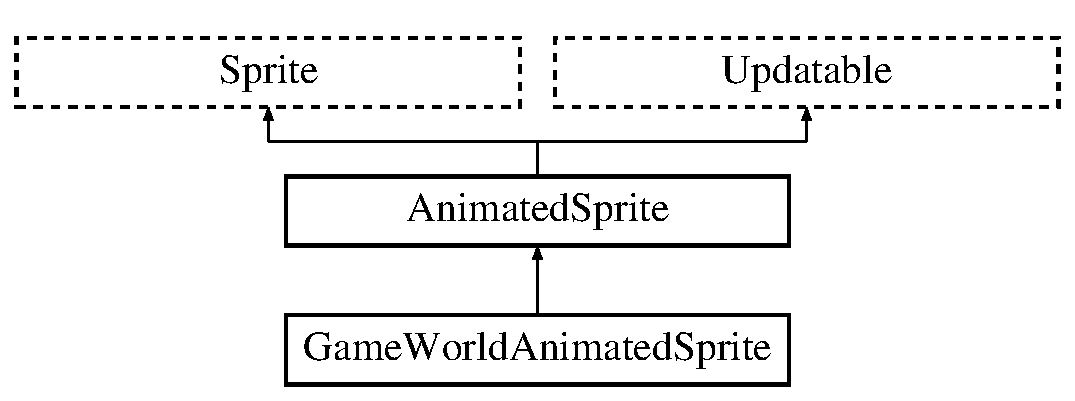
\includegraphics[height=3.000000cm]{class_animated_sprite}
\end{center}
\end{figure}
\subsection*{Public Member Functions}
\begin{DoxyCompactItemize}
\item 
\hyperlink{class_animated_sprite_a1147eb833593fa4c28854b96a84413a9}{Animated\+Sprite} ()
\begin{DoxyCompactList}\small\item\em Default Constructor. Values are not initialized 0.\end{DoxyCompactList}\item 
\hyperlink{class_animated_sprite_af8e492c2897e3335ba96149085f4d165}{Animated\+Sprite} (const sf\+::\+Texture \&texture)
\begin{DoxyCompactList}\small\item\em Initializes a new instance of the \hyperlink{class_animated_sprite}{Animated\+Sprite} class. Texture set to passed value. Position set to 0. \end{DoxyCompactList}\item 
\hyperlink{class_animated_sprite_ac17be6b9808193a6bcbdccd92b61e60e}{Animated\+Sprite} (const sf\+::\+Texture \&texture, \hyperlink{class_animation_set}{Animation\+Set} $\ast$animations)
\begin{DoxyCompactList}\small\item\em Initializes a new instance of the \hyperlink{class_animated_sprite}{Animated\+Sprite} class. Initializes texture to first frame of first animation. \end{DoxyCompactList}\item 
void \hyperlink{class_animated_sprite_ab73cac59a5415b0f08eb3963543d9bc8}{set\+Animating} (bool animating)
\begin{DoxyCompactList}\small\item\em Whether or not the animated sprite is currently playing an animation\end{DoxyCompactList}\item 
void \hyperlink{class_animated_sprite_a8ad3a9bac853b0b55fb3efd96c93a2d5}{set\+Current\+Frame} (unsigned int frame)
\begin{DoxyCompactList}\small\item\em sets the current frame (within the current animation) of the animated sprite \end{DoxyCompactList}\item 
void \hyperlink{class_animated_sprite_ab3a1384d836bc7f9b8580dccf33c2f1c}{set\+Animations} (\hyperlink{class_animation_set}{Animation\+Set} $\ast$animations)
\begin{DoxyCompactList}\small\item\em sets the animations of the sprite to the passed \hyperlink{class_animation_set}{Animation\+Set}. \end{DoxyCompactList}\item 
void \hyperlink{class_animated_sprite_a4dd9673ba304de36d69f15fe367a6e82}{set\+Animation\+Delay} (unsigned int speed)
\begin{DoxyCompactList}\small\item\em Sets the minimum time (in ms) between two animation frames. \end{DoxyCompactList}\item 
unsigned int \hyperlink{class_animated_sprite_a4d7dc2868007f5b15d3b25f7ab918155}{get\+Current\+Frame} ()
\begin{DoxyCompactList}\small\item\em returns the current frame of the current animation\end{DoxyCompactList}\item 
unsigned int \hyperlink{class_animated_sprite_abd64b160fdfae1d1eec67e017af5f375}{get\+Current\+Animation\+Id} ()
\begin{DoxyCompactList}\small\item\em returns the ID of the current animation \end{DoxyCompactList}\item 
unsigned int \hyperlink{class_animated_sprite_a23593d75ebc15e0e9969480239ae7830}{get\+Animation\+Delay} ()
\begin{DoxyCompactList}\small\item\em returns the minimum time (in ms) between two animation frames. \end{DoxyCompactList}\item 
bool \hyperlink{class_animated_sprite_a40beb8105603bf726270fb38400fe6bf}{is\+Animating} ()
\begin{DoxyCompactList}\small\item\em Determines whether this instance is animating. \end{DoxyCompactList}\item 
void \hyperlink{class_animated_sprite_a38725e0f5facf5d3d993500476790a9f}{run\+Animation} (unsigned int animation\+Id)
\begin{DoxyCompactList}\small\item\em begins a new animation from the first frame \end{DoxyCompactList}\item 
virtual void \hyperlink{class_animated_sprite_afdeda3e3030963a8ba290e23e48acc40}{update} (sf\+::\+Time current\+Time)
\begin{DoxyCompactList}\small\item\em Moves the next frame of the active animation if the sprite is animating \end{DoxyCompactList}\end{DoxyCompactItemize}
\subsection*{Protected Member Functions}
\begin{DoxyCompactItemize}
\item 
void \hyperlink{class_animated_sprite_a003d5c113b53ad5cb6c9836fb7b6d7c0}{Animated\+Sprite\+Init} (\hyperlink{class_animation_set}{Animation\+Set} $\ast$animations)
\begin{DoxyCompactList}\small\item\em Initializes properties to false, 0, or nullptr. Initializes animation set and sets texture to first animation frame if animation set is valid \end{DoxyCompactList}\end{DoxyCompactItemize}
\subsection*{Protected Attributes}
\begin{DoxyCompactItemize}
\item 
\mbox{\Hypertarget{class_animated_sprite_ae7c4fff66a7faf50d34e2864c0e21412}\label{class_animated_sprite_ae7c4fff66a7faf50d34e2864c0e21412}} 
std\+::vector$<$ std\+::vector$<$ sf\+::\+Int\+Rect $>$ $>$ $\ast$ {\bfseries animations}
\item 
\mbox{\Hypertarget{class_animated_sprite_a9f402cf567f00b4e9778cd078b1111d0}\label{class_animated_sprite_a9f402cf567f00b4e9778cd078b1111d0}} 
bool {\bfseries animating}
\item 
\mbox{\Hypertarget{class_animated_sprite_a5f59f0b90be8597ecc9f4b114dfbcf01}\label{class_animated_sprite_a5f59f0b90be8597ecc9f4b114dfbcf01}} 
unsigned int {\bfseries current\+Frame}
\item 
\mbox{\Hypertarget{class_animated_sprite_a9b346d42d71e889a20b9bcd32fab8470}\label{class_animated_sprite_a9b346d42d71e889a20b9bcd32fab8470}} 
unsigned int {\bfseries current\+Animation\+Id}
\item 
\mbox{\Hypertarget{class_animated_sprite_a1789989f7faf07dda742884b2251c256}\label{class_animated_sprite_a1789989f7faf07dda742884b2251c256}} 
std\+::vector$<$ sf\+::\+Int\+Rect $>$ $\ast$ {\bfseries current\+Animation}
\item 
\mbox{\Hypertarget{class_animated_sprite_a22ca1db04b4b746ee1363b57304dcb2b}\label{class_animated_sprite_a22ca1db04b4b746ee1363b57304dcb2b}} 
unsigned int {\bfseries animation\+Delay}
\end{DoxyCompactItemize}


\subsection{Detailed Description}
Sprite with the ability to display several animation states. 



\subsection{Constructor \& Destructor Documentation}
\mbox{\Hypertarget{class_animated_sprite_a1147eb833593fa4c28854b96a84413a9}\label{class_animated_sprite_a1147eb833593fa4c28854b96a84413a9}} 
\index{Animated\+Sprite@{Animated\+Sprite}!Animated\+Sprite@{Animated\+Sprite}}
\index{Animated\+Sprite@{Animated\+Sprite}!Animated\+Sprite@{Animated\+Sprite}}
\subsubsection{\texorpdfstring{Animated\+Sprite()}{AnimatedSprite()}\hspace{0.1cm}{\footnotesize\ttfamily [1/3]}}
{\footnotesize\ttfamily Animated\+Sprite\+::\+Animated\+Sprite (\begin{DoxyParamCaption}{ }\end{DoxyParamCaption})}



Default Constructor. Values are not initialized 0.

\mbox{\Hypertarget{class_animated_sprite_af8e492c2897e3335ba96149085f4d165}\label{class_animated_sprite_af8e492c2897e3335ba96149085f4d165}} 
\index{Animated\+Sprite@{Animated\+Sprite}!Animated\+Sprite@{Animated\+Sprite}}
\index{Animated\+Sprite@{Animated\+Sprite}!Animated\+Sprite@{Animated\+Sprite}}
\subsubsection{\texorpdfstring{Animated\+Sprite()}{AnimatedSprite()}\hspace{0.1cm}{\footnotesize\ttfamily [2/3]}}
{\footnotesize\ttfamily Animated\+Sprite\+::\+Animated\+Sprite (\begin{DoxyParamCaption}\item[{const sf\+::\+Texture \&}]{texture }\end{DoxyParamCaption})\hspace{0.3cm}{\ttfamily [explicit]}}



Initializes a new instance of the \hyperlink{class_animated_sprite}{Animated\+Sprite} class. Texture set to passed value. Position set to 0. 


\begin{DoxyParams}{Parameters}
{\em texture} & The texture.\\
\hline
\end{DoxyParams}
\mbox{\Hypertarget{class_animated_sprite_ac17be6b9808193a6bcbdccd92b61e60e}\label{class_animated_sprite_ac17be6b9808193a6bcbdccd92b61e60e}} 
\index{Animated\+Sprite@{Animated\+Sprite}!Animated\+Sprite@{Animated\+Sprite}}
\index{Animated\+Sprite@{Animated\+Sprite}!Animated\+Sprite@{Animated\+Sprite}}
\subsubsection{\texorpdfstring{Animated\+Sprite()}{AnimatedSprite()}\hspace{0.1cm}{\footnotesize\ttfamily [3/3]}}
{\footnotesize\ttfamily Animated\+Sprite\+::\+Animated\+Sprite (\begin{DoxyParamCaption}\item[{const sf\+::\+Texture \&}]{texture,  }\item[{\hyperlink{class_animation_set}{Animation\+Set} $\ast$}]{animations }\end{DoxyParamCaption})}



Initializes a new instance of the \hyperlink{class_animated_sprite}{Animated\+Sprite} class. Initializes texture to first frame of first animation. 


\begin{DoxyParams}{Parameters}
{\em texture} & texture representing the animation sheet.\\
\hline
{\em animations} & The animations.\\
\hline
\end{DoxyParams}


\subsection{Member Function Documentation}
\mbox{\Hypertarget{class_animated_sprite_a003d5c113b53ad5cb6c9836fb7b6d7c0}\label{class_animated_sprite_a003d5c113b53ad5cb6c9836fb7b6d7c0}} 
\index{Animated\+Sprite@{Animated\+Sprite}!Animated\+Sprite\+Init@{Animated\+Sprite\+Init}}
\index{Animated\+Sprite\+Init@{Animated\+Sprite\+Init}!Animated\+Sprite@{Animated\+Sprite}}
\subsubsection{\texorpdfstring{Animated\+Sprite\+Init()}{AnimatedSpriteInit()}}
{\footnotesize\ttfamily void Animated\+Sprite\+::\+Animated\+Sprite\+Init (\begin{DoxyParamCaption}\item[{\hyperlink{class_animation_set}{Animation\+Set} $\ast$}]{animations }\end{DoxyParamCaption})\hspace{0.3cm}{\ttfamily [protected]}}



Initializes properties to false, 0, or nullptr. Initializes animation set and sets texture to first animation frame if animation set is valid 


\begin{DoxyParams}{Parameters}
{\em animations} & animation set for the sprite. If this value is set to a valid animation then the texture of the sprite is set to the first frame of the first animation.\\
\hline
\end{DoxyParams}
\mbox{\Hypertarget{class_animated_sprite_a23593d75ebc15e0e9969480239ae7830}\label{class_animated_sprite_a23593d75ebc15e0e9969480239ae7830}} 
\index{Animated\+Sprite@{Animated\+Sprite}!get\+Animation\+Delay@{get\+Animation\+Delay}}
\index{get\+Animation\+Delay@{get\+Animation\+Delay}!Animated\+Sprite@{Animated\+Sprite}}
\subsubsection{\texorpdfstring{get\+Animation\+Delay()}{getAnimationDelay()}}
{\footnotesize\ttfamily unsigned int Animated\+Sprite\+::get\+Animation\+Delay (\begin{DoxyParamCaption}{ }\end{DoxyParamCaption})}



returns the minimum time (in ms) between two animation frames. 

\begin{DoxyReturn}{Returns}
The minimum time (in ms) between two animation frames.
\end{DoxyReturn}
\mbox{\Hypertarget{class_animated_sprite_abd64b160fdfae1d1eec67e017af5f375}\label{class_animated_sprite_abd64b160fdfae1d1eec67e017af5f375}} 
\index{Animated\+Sprite@{Animated\+Sprite}!get\+Current\+Animation\+Id@{get\+Current\+Animation\+Id}}
\index{get\+Current\+Animation\+Id@{get\+Current\+Animation\+Id}!Animated\+Sprite@{Animated\+Sprite}}
\subsubsection{\texorpdfstring{get\+Current\+Animation\+Id()}{getCurrentAnimationId()}}
{\footnotesize\ttfamily unsigned int Animated\+Sprite\+::get\+Current\+Animation\+Id (\begin{DoxyParamCaption}{ }\end{DoxyParamCaption})}



returns the ID of the current animation 

\begin{DoxyReturn}{Returns}
ID of the current animation.
\end{DoxyReturn}
\mbox{\Hypertarget{class_animated_sprite_a4d7dc2868007f5b15d3b25f7ab918155}\label{class_animated_sprite_a4d7dc2868007f5b15d3b25f7ab918155}} 
\index{Animated\+Sprite@{Animated\+Sprite}!get\+Current\+Frame@{get\+Current\+Frame}}
\index{get\+Current\+Frame@{get\+Current\+Frame}!Animated\+Sprite@{Animated\+Sprite}}
\subsubsection{\texorpdfstring{get\+Current\+Frame()}{getCurrentFrame()}}
{\footnotesize\ttfamily unsigned int Animated\+Sprite\+::get\+Current\+Frame (\begin{DoxyParamCaption}{ }\end{DoxyParamCaption})}



returns the current frame of the current animation

\mbox{\Hypertarget{class_animated_sprite_a40beb8105603bf726270fb38400fe6bf}\label{class_animated_sprite_a40beb8105603bf726270fb38400fe6bf}} 
\index{Animated\+Sprite@{Animated\+Sprite}!is\+Animating@{is\+Animating}}
\index{is\+Animating@{is\+Animating}!Animated\+Sprite@{Animated\+Sprite}}
\subsubsection{\texorpdfstring{is\+Animating()}{isAnimating()}}
{\footnotesize\ttfamily bool Animated\+Sprite\+::is\+Animating (\begin{DoxyParamCaption}{ }\end{DoxyParamCaption})}



Determines whether this instance is animating. 

\begin{DoxyReturn}{Returns}
{\ttfamily true} if this instance is animating; otherwise, {\ttfamily false}. 
\end{DoxyReturn}
\mbox{\Hypertarget{class_animated_sprite_a38725e0f5facf5d3d993500476790a9f}\label{class_animated_sprite_a38725e0f5facf5d3d993500476790a9f}} 
\index{Animated\+Sprite@{Animated\+Sprite}!run\+Animation@{run\+Animation}}
\index{run\+Animation@{run\+Animation}!Animated\+Sprite@{Animated\+Sprite}}
\subsubsection{\texorpdfstring{run\+Animation()}{runAnimation()}}
{\footnotesize\ttfamily void Animated\+Sprite\+::run\+Animation (\begin{DoxyParamCaption}\item[{unsigned int}]{animation\+Id }\end{DoxyParamCaption})}



begins a new animation from the first frame 


\begin{DoxyParams}{Parameters}
{\em animation\+Id} & the index of the animation to begin.\\
\hline
\end{DoxyParams}
\mbox{\Hypertarget{class_animated_sprite_ab73cac59a5415b0f08eb3963543d9bc8}\label{class_animated_sprite_ab73cac59a5415b0f08eb3963543d9bc8}} 
\index{Animated\+Sprite@{Animated\+Sprite}!set\+Animating@{set\+Animating}}
\index{set\+Animating@{set\+Animating}!Animated\+Sprite@{Animated\+Sprite}}
\subsubsection{\texorpdfstring{set\+Animating()}{setAnimating()}}
{\footnotesize\ttfamily void Animated\+Sprite\+::set\+Animating (\begin{DoxyParamCaption}\item[{bool}]{animating }\end{DoxyParamCaption})}



Whether or not the animated sprite is currently playing an animation

\mbox{\Hypertarget{class_animated_sprite_a4dd9673ba304de36d69f15fe367a6e82}\label{class_animated_sprite_a4dd9673ba304de36d69f15fe367a6e82}} 
\index{Animated\+Sprite@{Animated\+Sprite}!set\+Animation\+Delay@{set\+Animation\+Delay}}
\index{set\+Animation\+Delay@{set\+Animation\+Delay}!Animated\+Sprite@{Animated\+Sprite}}
\subsubsection{\texorpdfstring{set\+Animation\+Delay()}{setAnimationDelay()}}
{\footnotesize\ttfamily void Animated\+Sprite\+::set\+Animation\+Delay (\begin{DoxyParamCaption}\item[{unsigned int}]{delay }\end{DoxyParamCaption})}



Sets the minimum time (in ms) between two animation frames. 


\begin{DoxyParams}{Parameters}
{\em delay} & Minimum time (in ms) between two animation frames.\\
\hline
\end{DoxyParams}
\mbox{\Hypertarget{class_animated_sprite_ab3a1384d836bc7f9b8580dccf33c2f1c}\label{class_animated_sprite_ab3a1384d836bc7f9b8580dccf33c2f1c}} 
\index{Animated\+Sprite@{Animated\+Sprite}!set\+Animations@{set\+Animations}}
\index{set\+Animations@{set\+Animations}!Animated\+Sprite@{Animated\+Sprite}}
\subsubsection{\texorpdfstring{set\+Animations()}{setAnimations()}}
{\footnotesize\ttfamily void Animated\+Sprite\+::set\+Animations (\begin{DoxyParamCaption}\item[{\hyperlink{class_animation_set}{Animation\+Set} $\ast$}]{animation\+Set }\end{DoxyParamCaption})}



sets the animations of the sprite to the passed \hyperlink{class_animation_set}{Animation\+Set}. 


\begin{DoxyParams}{Parameters}
{\em animation\+Set} & The animation set.\\
\hline
\end{DoxyParams}
\mbox{\Hypertarget{class_animated_sprite_a8ad3a9bac853b0b55fb3efd96c93a2d5}\label{class_animated_sprite_a8ad3a9bac853b0b55fb3efd96c93a2d5}} 
\index{Animated\+Sprite@{Animated\+Sprite}!set\+Current\+Frame@{set\+Current\+Frame}}
\index{set\+Current\+Frame@{set\+Current\+Frame}!Animated\+Sprite@{Animated\+Sprite}}
\subsubsection{\texorpdfstring{set\+Current\+Frame()}{setCurrentFrame()}}
{\footnotesize\ttfamily void Animated\+Sprite\+::set\+Current\+Frame (\begin{DoxyParamCaption}\item[{unsigned int}]{frame }\end{DoxyParamCaption})}



sets the current frame (within the current animation) of the animated sprite 


\begin{DoxyParams}{Parameters}
{\em frame} & The frame.\\
\hline
\end{DoxyParams}
\mbox{\Hypertarget{class_animated_sprite_afdeda3e3030963a8ba290e23e48acc40}\label{class_animated_sprite_afdeda3e3030963a8ba290e23e48acc40}} 
\index{Animated\+Sprite@{Animated\+Sprite}!update@{update}}
\index{update@{update}!Animated\+Sprite@{Animated\+Sprite}}
\subsubsection{\texorpdfstring{update()}{update()}}
{\footnotesize\ttfamily void Animated\+Sprite\+::update (\begin{DoxyParamCaption}\item[{sf\+::\+Time}]{current\+Time }\end{DoxyParamCaption})\hspace{0.3cm}{\ttfamily [virtual]}}



Moves the next frame of the active animation if the sprite is animating 


\begin{DoxyParams}{Parameters}
{\em current\+Time} & The current time.\\
\hline
\end{DoxyParams}


Implements \hyperlink{class_updatable}{Updatable}.



Reimplemented in \hyperlink{class_game_world_animated_sprite_a6fab62c5ed11541027a88c695a8b6147}{Game\+World\+Animated\+Sprite}.



The documentation for this class was generated from the following files\+:\begin{DoxyCompactItemize}
\item 
E\+:/\+Programing/\+Programing/\+Cpp/\+Game\+Backbone/\+Game\+Backbone/Animated\+Sprite.\+h\item 
E\+:/\+Programing/\+Programing/\+Cpp/\+Game\+Backbone/\+Game\+Backbone/Animated\+Sprite.\+cpp\end{DoxyCompactItemize}

\hypertarget{class_animation_set}{}\section{Animation\+Set Class Reference}
\label{class_animation_set}\index{Animation\+Set@{Animation\+Set}}


A groups of Animation frames used by animated sprites to determine animation loops 




{\ttfamily \#include $<$Animation\+Set.\+h$>$}

\subsection*{Public Member Functions}
\begin{DoxyCompactItemize}
\item 
\hyperlink{class_animation_set_a4291450987a71b6923ecdc44d38f3647}{Animation\+Set} (unsigned int rows, unsigned int cols)
\begin{DoxyCompactList}\small\item\em Initializes a new instance of the \hyperlink{class_animation_set}{Animation\+Set} class. \end{DoxyCompactList}\item 
\hyperlink{class_animation_set_a1a7cce6f8664911363d621ec01f022e6}{Animation\+Set} (const std\+::vector$<$ std\+::vector$<$ unsigned int $>$$>$ \&frame\+Animations, unsigned int texture\+Width, unsigned int texture\+Height, unsigned int rows, unsigned int cols)
\begin{DoxyCompactList}\small\item\em Initializes a new instance of the \hyperlink{class_animation_set}{Animation\+Set} class. \end{DoxyCompactList}\item 
void \hyperlink{class_animation_set_ab673697a6a87e0d62cc9d8da5912e633}{frames\+To\+Rects} (const std\+::vector$<$ std\+::vector$<$ unsigned int $>$$>$ \&frame\+Animations, unsigned int texture\+Width, unsigned int texture\+Height)
\begin{DoxyCompactList}\small\item\em Converts a full set of animations in the frame number format to the texture\+Rect format \end{DoxyCompactList}\item 
void \hyperlink{class_animation_set_a6c48243cd06f90f7b21c792f7f092a83}{clear\+Animations} ()
\begin{DoxyCompactList}\small\item\em Clears all animations. \end{DoxyCompactList}\item 
std\+::vector$<$ std\+::vector$<$ sf\+::\+Int\+Rect $>$ $>$ $\ast$ \hyperlink{class_animation_set_ae523b9c1f7702b1ebe02662078a8f701}{get\+Animations} ()
\begin{DoxyCompactList}\small\item\em returns a const pointer to the vector of animations \end{DoxyCompactList}\end{DoxyCompactItemize}
\subsection*{Protected Attributes}
\begin{DoxyCompactItemize}
\item 
\mbox{\Hypertarget{class_animation_set_a9e31574676175d9d5dc36ef5facf7150}\label{class_animation_set_a9e31574676175d9d5dc36ef5facf7150}} 
unsigned int {\bfseries rows}
\item 
\mbox{\Hypertarget{class_animation_set_ababecc4cc5e80e68da53a9aabbef1c88}\label{class_animation_set_ababecc4cc5e80e68da53a9aabbef1c88}} 
unsigned int {\bfseries cols}
\item 
\mbox{\Hypertarget{class_animation_set_aa36a8a16f556bb3609c8dc2b64030387}\label{class_animation_set_aa36a8a16f556bb3609c8dc2b64030387}} 
std\+::vector$<$ std\+::vector$<$ sf\+::\+Int\+Rect $>$ $>$ {\bfseries animations}
\end{DoxyCompactItemize}


\subsection{Detailed Description}
A groups of Animation frames used by animated sprites to determine animation loops



\subsection{Constructor \& Destructor Documentation}
\mbox{\Hypertarget{class_animation_set_a4291450987a71b6923ecdc44d38f3647}\label{class_animation_set_a4291450987a71b6923ecdc44d38f3647}} 
\index{Animation\+Set@{Animation\+Set}!Animation\+Set@{Animation\+Set}}
\index{Animation\+Set@{Animation\+Set}!Animation\+Set@{Animation\+Set}}
\subsubsection{\texorpdfstring{Animation\+Set()}{AnimationSet()}\hspace{0.1cm}{\footnotesize\ttfamily [1/2]}}
{\footnotesize\ttfamily Animation\+Set\+::\+Animation\+Set (\begin{DoxyParamCaption}\item[{unsigned int}]{rows,  }\item[{unsigned int}]{cols }\end{DoxyParamCaption})}



Initializes a new instance of the \hyperlink{class_animation_set}{Animation\+Set} class. 


\begin{DoxyParams}{Parameters}
{\em rows} & The number of rows in the sprite sheet.\\
\hline
{\em cols} & The number of columns in the sprite sheet.\\
\hline
\end{DoxyParams}
\mbox{\Hypertarget{class_animation_set_a1a7cce6f8664911363d621ec01f022e6}\label{class_animation_set_a1a7cce6f8664911363d621ec01f022e6}} 
\index{Animation\+Set@{Animation\+Set}!Animation\+Set@{Animation\+Set}}
\index{Animation\+Set@{Animation\+Set}!Animation\+Set@{Animation\+Set}}
\subsubsection{\texorpdfstring{Animation\+Set()}{AnimationSet()}\hspace{0.1cm}{\footnotesize\ttfamily [2/2]}}
{\footnotesize\ttfamily Animation\+Set\+::\+Animation\+Set (\begin{DoxyParamCaption}\item[{const std\+::vector$<$ std\+::vector$<$ unsigned int $>$$>$ \&}]{frame\+Animations,  }\item[{unsigned int}]{texture\+Width,  }\item[{unsigned int}]{texture\+Height,  }\item[{unsigned int}]{rows,  }\item[{unsigned int}]{cols }\end{DoxyParamCaption})}



Initializes a new instance of the \hyperlink{class_animation_set}{Animation\+Set} class. 


\begin{DoxyParams}{Parameters}
{\em frame\+Animations} & Arrays of frame numbers for each animation in the set. Each array corresponds to the animation of the same index.\\
\hline
{\em texture\+Width} & Width of the texture.\\
\hline
{\em texture\+Height} & Height of the texture.\\
\hline
{\em rows} & The number of rows in the sprite sheet.\\
\hline
{\em cols} & The number of columns in the sprite sheet.\\
\hline
\end{DoxyParams}


\subsection{Member Function Documentation}
\mbox{\Hypertarget{class_animation_set_a6c48243cd06f90f7b21c792f7f092a83}\label{class_animation_set_a6c48243cd06f90f7b21c792f7f092a83}} 
\index{Animation\+Set@{Animation\+Set}!clear\+Animations@{clear\+Animations}}
\index{clear\+Animations@{clear\+Animations}!Animation\+Set@{Animation\+Set}}
\subsubsection{\texorpdfstring{clear\+Animations()}{clearAnimations()}}
{\footnotesize\ttfamily void Animation\+Set\+::clear\+Animations (\begin{DoxyParamCaption}{ }\end{DoxyParamCaption})}



Clears all animations. 

\mbox{\Hypertarget{class_animation_set_ab673697a6a87e0d62cc9d8da5912e633}\label{class_animation_set_ab673697a6a87e0d62cc9d8da5912e633}} 
\index{Animation\+Set@{Animation\+Set}!frames\+To\+Rects@{frames\+To\+Rects}}
\index{frames\+To\+Rects@{frames\+To\+Rects}!Animation\+Set@{Animation\+Set}}
\subsubsection{\texorpdfstring{frames\+To\+Rects()}{framesToRects()}}
{\footnotesize\ttfamily void Animation\+Set\+::frames\+To\+Rects (\begin{DoxyParamCaption}\item[{const std\+::vector$<$ std\+::vector$<$ unsigned int $>$$>$ \&}]{frame\+Animations,  }\item[{unsigned int}]{texture\+Width,  }\item[{unsigned int}]{texture\+Height }\end{DoxyParamCaption})}



Converts a full set of animations in the frame number format to the texture\+Rect format 


\begin{DoxyParams}{Parameters}
{\em frame\+Animations} & Animation represented by frame numbers.\\
\hline
{\em texture\+Width} & Width of the sprite sheet texture.\\
\hline
{\em texture\+Height} & Height of the sprite sheet texture.\\
\hline
\end{DoxyParams}
\mbox{\Hypertarget{class_animation_set_ae523b9c1f7702b1ebe02662078a8f701}\label{class_animation_set_ae523b9c1f7702b1ebe02662078a8f701}} 
\index{Animation\+Set@{Animation\+Set}!get\+Animations@{get\+Animations}}
\index{get\+Animations@{get\+Animations}!Animation\+Set@{Animation\+Set}}
\subsubsection{\texorpdfstring{get\+Animations()}{getAnimations()}}
{\footnotesize\ttfamily std\+::vector$<$ std\+::vector$<$ sf\+::\+Int\+Rect $>$ $>$ $\ast$ Animation\+Set\+::get\+Animations (\begin{DoxyParamCaption}{ }\end{DoxyParamCaption})}



returns a const pointer to the vector of animations 

\begin{DoxyReturn}{Returns}

\end{DoxyReturn}


The documentation for this class was generated from the following files\+:\begin{DoxyCompactItemize}
\item 
E\+:/\+Programing/\+Programing/\+Cpp/\+Game\+Backbone/\+Game\+Backbone/Animation\+Set.\+h\item 
E\+:/\+Programing/\+Programing/\+Cpp/\+Game\+Backbone/\+Game\+Backbone/Animation\+Set.\+cpp\end{DoxyCompactItemize}

\hypertarget{class_array3_d}{}\section{Array3D$<$ template\+Class $>$ Class Template Reference}
\label{class_array3_d}\index{Array3\+D$<$ template\+Class $>$@{Array3\+D$<$ template\+Class $>$}}


Store any type in a three dimensional array 




{\ttfamily \#include $<$Array3\+D.\+h$>$}

\subsection*{Public Member Functions}
\begin{DoxyCompactItemize}
\item 
\hyperlink{class_array3_d_a86765d4b26c76555b35279d42a69158a}{Array3D} ()
\begin{DoxyCompactList}\small\item\em creates a 3D array with dimensions of 100 $\ast$ 100 $\ast$ 100 \end{DoxyCompactList}\item 
\hyperlink{class_array3_d_a16a7c8e4de7c1529f4d72c00d2f5b8f9}{Array3D} (unsigned int dimensions)
\item 
\mbox{\Hypertarget{class_array3_d_a603b0ad73fd7bb2a28e08538bb8e2ad6}\label{class_array3_d_a603b0ad73fd7bb2a28e08538bb8e2ad6}} 
{\bfseries Array3D} (unsigned int x\+Lenght, unsigned int y\+Length, unsigned int z\+Length)
\item 
void \hyperlink{class_array3_d_ab10ba3c75901c55b3d7cd2f58f6d6bde}{set\+Value\+At} (unsigned int x, unsigned int y, unsigned int z, template\+Class value)
\begin{DoxyCompactList}\small\item\em sets the value of the selected array index to the passed value\end{DoxyCompactList}\item 
template\+Class \hyperlink{class_array3_d_ac16b3ce3f37d597033a7b7fd1fdb5e41}{get\+Value\+At} (unsigned int x, unsigned int y, unsigned int z)
\begin{DoxyCompactList}\small\item\em returns the weight of the specified array index \end{DoxyCompactList}\item 
template\+Class \hyperlink{class_array3_d_ac1539b1f9907ae9996178b968e43c53c}{get\+Value\+At} (sf\+::\+Vector3i coordinate)
\begin{DoxyCompactList}\small\item\em returns the weight of the specified array index. \end{DoxyCompactList}\item 
unsigned int \hyperlink{class_array3_d_a5c406bcb6868cb65acb6ac1f593d743e}{get\+Array\+SizeX} ()
\begin{DoxyCompactList}\small\item\em summary$>$ returns the y dimension of the array\end{DoxyCompactList}\item 
unsigned int \hyperlink{class_array3_d_a1d60c3290d17e30e1e5854f296bba68b}{get\+Array\+SizeY} ()
\begin{DoxyCompactList}\small\item\em summary$>$ returns the z dimension of the grid\end{DoxyCompactList}\item 
\mbox{\Hypertarget{class_array3_d_a6223fa080e3dfef08b48f893fad066ad}\label{class_array3_d_a6223fa080e3dfef08b48f893fad066ad}} 
unsigned int {\bfseries get\+Array\+SizeZ} ()
\item 
void \hyperlink{class_array3_d_a0bc535dddbd5c2e5597fc967aa0e4a0e}{init\+All\+Values} (template\+Class value)
\begin{DoxyCompactList}\small\item\em Initializes all values of the array to the passed value. Existing values are overwritten. \end{DoxyCompactList}\end{DoxyCompactItemize}


\subsection{Detailed Description}
\subsubsection*{template$<$class template\+Class$>$\newline
class Array3\+D$<$ template\+Class $>$}

Store any type in a three dimensional array



\subsection{Constructor \& Destructor Documentation}
\mbox{\Hypertarget{class_array3_d_a86765d4b26c76555b35279d42a69158a}\label{class_array3_d_a86765d4b26c76555b35279d42a69158a}} 
\index{Array3D@{Array3D}!Array3D@{Array3D}}
\index{Array3D@{Array3D}!Array3D@{Array3D}}
\subsubsection{\texorpdfstring{Array3\+D()}{Array3D()}\hspace{0.1cm}{\footnotesize\ttfamily [1/2]}}
{\footnotesize\ttfamily template$<$class template\+Class $>$ \\
\hyperlink{class_array3_d}{Array3D}$<$ template\+Class $>$\+::\hyperlink{class_array3_d}{Array3D} (\begin{DoxyParamCaption}{ }\end{DoxyParamCaption})\hspace{0.3cm}{\ttfamily [inline]}}



creates a 3D array with dimensions of 100 $\ast$ 100 $\ast$ 100 

summary$>$ creates a cube 3D array with the passed width.

param name = \char`\"{}dimensions\char`\"{}$>$ size of the width of the array cube\mbox{\Hypertarget{class_array3_d_a16a7c8e4de7c1529f4d72c00d2f5b8f9}\label{class_array3_d_a16a7c8e4de7c1529f4d72c00d2f5b8f9}} 
\index{Array3D@{Array3D}!Array3D@{Array3D}}
\index{Array3D@{Array3D}!Array3D@{Array3D}}
\subsubsection{\texorpdfstring{Array3\+D()}{Array3D()}\hspace{0.1cm}{\footnotesize\ttfamily [2/2]}}
{\footnotesize\ttfamily template$<$class template\+Class $>$ \\
\hyperlink{class_array3_d}{Array3D}$<$ template\+Class $>$\+::\hyperlink{class_array3_d}{Array3D} (\begin{DoxyParamCaption}\item[{unsigned int}]{dimensions }\end{DoxyParamCaption})\hspace{0.3cm}{\ttfamily [inline]}, {\ttfamily [explicit]}}

summary$>$ creates a 3D array with passed x , y and z dimensions.

param name = \char`\"{}x\+Dim\char`\"{}$>$size of the array in the x dimension

param name = \char`\"{}y\+Dim\char`\"{}$>$size of the array in the y dimension

param name = \char`\"{}z\+Dim\char`\"{}$>$size of the array in the z dimension

\subsection{Member Function Documentation}
\mbox{\Hypertarget{class_array3_d_a5c406bcb6868cb65acb6ac1f593d743e}\label{class_array3_d_a5c406bcb6868cb65acb6ac1f593d743e}} 
\index{Array3D@{Array3D}!get\+Array\+SizeX@{get\+Array\+SizeX}}
\index{get\+Array\+SizeX@{get\+Array\+SizeX}!Array3D@{Array3D}}
\subsubsection{\texorpdfstring{get\+Array\+Size\+X()}{getArraySizeX()}}
{\footnotesize\ttfamily template$<$class template\+Class $>$ \\
unsigned int \hyperlink{class_array3_d}{Array3D}$<$ template\+Class $>$\+::get\+Array\+SizeX (\begin{DoxyParamCaption}{ }\end{DoxyParamCaption})\hspace{0.3cm}{\ttfamily [inline]}}



summary$>$ returns the y dimension of the array

\mbox{\Hypertarget{class_array3_d_a1d60c3290d17e30e1e5854f296bba68b}\label{class_array3_d_a1d60c3290d17e30e1e5854f296bba68b}} 
\index{Array3D@{Array3D}!get\+Array\+SizeY@{get\+Array\+SizeY}}
\index{get\+Array\+SizeY@{get\+Array\+SizeY}!Array3D@{Array3D}}
\subsubsection{\texorpdfstring{get\+Array\+Size\+Y()}{getArraySizeY()}}
{\footnotesize\ttfamily template$<$class template\+Class $>$ \\
unsigned int \hyperlink{class_array3_d}{Array3D}$<$ template\+Class $>$\+::get\+Array\+SizeY (\begin{DoxyParamCaption}{ }\end{DoxyParamCaption})\hspace{0.3cm}{\ttfamily [inline]}}



summary$>$ returns the z dimension of the grid

\mbox{\Hypertarget{class_array3_d_ac16b3ce3f37d597033a7b7fd1fdb5e41}\label{class_array3_d_ac16b3ce3f37d597033a7b7fd1fdb5e41}} 
\index{Array3D@{Array3D}!get\+Value\+At@{get\+Value\+At}}
\index{get\+Value\+At@{get\+Value\+At}!Array3D@{Array3D}}
\subsubsection{\texorpdfstring{get\+Value\+At()}{getValueAt()}\hspace{0.1cm}{\footnotesize\ttfamily [1/2]}}
{\footnotesize\ttfamily template$<$class template\+Class $>$ \\
template\+Class \hyperlink{class_array3_d}{Array3D}$<$ template\+Class $>$\+::get\+Value\+At (\begin{DoxyParamCaption}\item[{unsigned int}]{x,  }\item[{unsigned int}]{y,  }\item[{unsigned int}]{z }\end{DoxyParamCaption})\hspace{0.3cm}{\ttfamily [inline]}}



returns the weight of the specified array index 

param name = \char`\"{}x\char`\"{}$>$x position of the element to return

param name = \char`\"{}y\char`\"{}$>$y position of the element to return

param name = \char`\"{}z\char`\"{}$>$z position of the element to return

\begin{DoxyReturn}{Returns}
The element stored at the passed coordinates
\end{DoxyReturn}
\mbox{\Hypertarget{class_array3_d_ac1539b1f9907ae9996178b968e43c53c}\label{class_array3_d_ac1539b1f9907ae9996178b968e43c53c}} 
\index{Array3D@{Array3D}!get\+Value\+At@{get\+Value\+At}}
\index{get\+Value\+At@{get\+Value\+At}!Array3D@{Array3D}}
\subsubsection{\texorpdfstring{get\+Value\+At()}{getValueAt()}\hspace{0.1cm}{\footnotesize\ttfamily [2/2]}}
{\footnotesize\ttfamily template$<$class template\+Class $>$ \\
template\+Class \hyperlink{class_array3_d}{Array3D}$<$ template\+Class $>$\+::get\+Value\+At (\begin{DoxyParamCaption}\item[{sf\+::\+Vector3i}]{coordinate }\end{DoxyParamCaption})\hspace{0.3cm}{\ttfamily [inline]}}



returns the weight of the specified array index. 


\begin{DoxyParams}{Parameters}
{\em coordinate} & The 3d position of the element to return.\\
\hline
\end{DoxyParams}
\begin{DoxyReturn}{Returns}
The element stored at the passed coordinates
\end{DoxyReturn}
summary$>$ returns the x dimension of the array\mbox{\Hypertarget{class_array3_d_a0bc535dddbd5c2e5597fc967aa0e4a0e}\label{class_array3_d_a0bc535dddbd5c2e5597fc967aa0e4a0e}} 
\index{Array3D@{Array3D}!init\+All\+Values@{init\+All\+Values}}
\index{init\+All\+Values@{init\+All\+Values}!Array3D@{Array3D}}
\subsubsection{\texorpdfstring{init\+All\+Values()}{initAllValues()}}
{\footnotesize\ttfamily template$<$class template\+Class $>$ \\
void \hyperlink{class_array3_d}{Array3D}$<$ template\+Class $>$\+::init\+All\+Values (\begin{DoxyParamCaption}\item[{template\+Class}]{value }\end{DoxyParamCaption})\hspace{0.3cm}{\ttfamily [inline]}}



Initializes all values of the array to the passed value. Existing values are overwritten. 

param name = \char`\"{}value\char`\"{}$>$ new value for every element in the array \mbox{\Hypertarget{class_array3_d_ab10ba3c75901c55b3d7cd2f58f6d6bde}\label{class_array3_d_ab10ba3c75901c55b3d7cd2f58f6d6bde}} 
\index{Array3D@{Array3D}!set\+Value\+At@{set\+Value\+At}}
\index{set\+Value\+At@{set\+Value\+At}!Array3D@{Array3D}}
\subsubsection{\texorpdfstring{set\+Value\+At()}{setValueAt()}}
{\footnotesize\ttfamily template$<$class template\+Class $>$ \\
void \hyperlink{class_array3_d}{Array3D}$<$ template\+Class $>$\+::set\+Value\+At (\begin{DoxyParamCaption}\item[{unsigned int}]{x,  }\item[{unsigned int}]{y,  }\item[{unsigned int}]{z,  }\item[{template\+Class}]{value }\end{DoxyParamCaption})\hspace{0.3cm}{\ttfamily [inline]}}



sets the value of the selected array index to the passed value

param name = \char`\"{}x\char`\"{}$>$x coordinate of the array index to change

param name = \char`\"{}y\char`\"{}$>$y coordinate of the array index to change

param name = \char`\"{}z\char`\"{}$>$z coordinate of the array index to change

param name = \char`\"{}value\char`\"{}$>$ new value for the passed array index

The documentation for this class was generated from the following file\+:\begin{DoxyCompactItemize}
\item 
E\+:/\+Programing/\+Programing/\+Cpp/\+Game\+Backbone/\+Game\+Backbone/Array3\+D.\+h\end{DoxyCompactItemize}

\hypertarget{class_compound_sprite}{}\section{Compound\+Sprite Class Reference}
\label{class_compound_sprite}\index{Compound\+Sprite@{Compound\+Sprite}}


Controls several sprites and animated sprites as one logical unit.  




{\ttfamily \#include $<$Compound\+Sprite.\+h$>$}

Inheritance diagram for Compound\+Sprite\+:\begin{figure}[H]
\begin{center}
\leavevmode
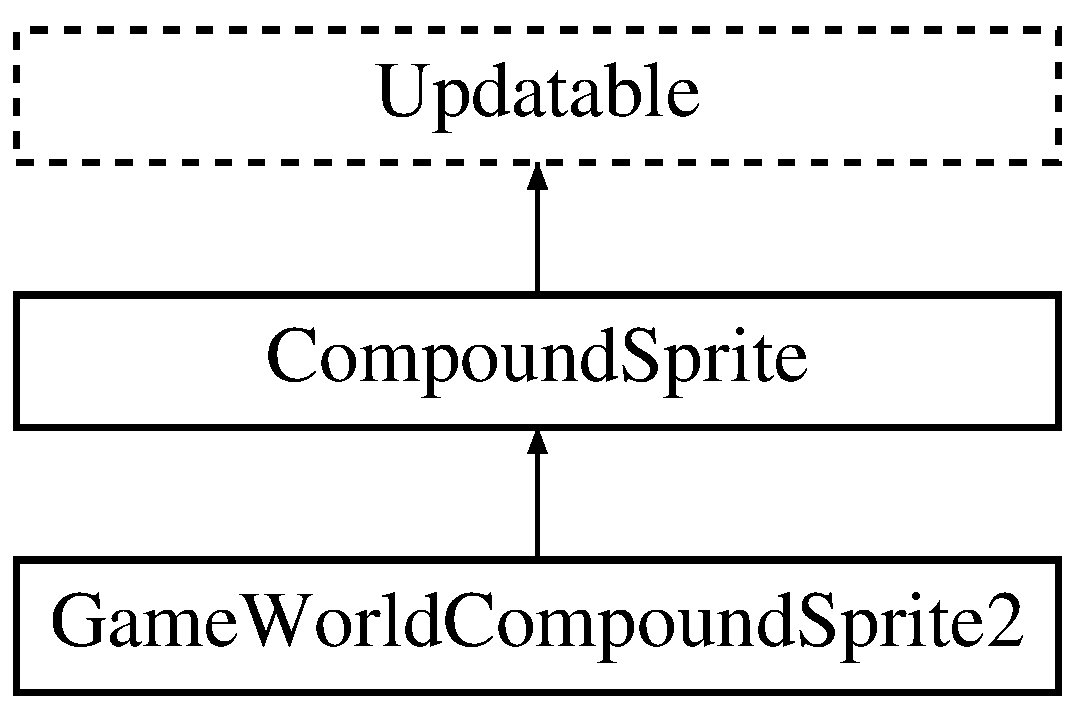
\includegraphics[height=3.000000cm]{class_compound_sprite}
\end{center}
\end{figure}
\subsection*{Public Member Functions}
\begin{DoxyCompactItemize}
\item 
\hyperlink{class_compound_sprite_ae9cc3d47da7d32e94b4c96c1ca55322c}{Compound\+Sprite} (const std\+::vector$<$ sf\+::\+Sprite $\ast$$>$ \&sprites, const std\+::vector$<$ \hyperlink{class_animated_sprite}{Animated\+Sprite} $\ast$$>$ \&animated\+Sprites)
\begin{DoxyCompactList}\small\item\em Initializes a new instance of the \hyperlink{class_compound_sprite}{Compound\+Sprite} class. Stores the passed groups of sf\+::\+Sprite and \hyperlink{class_animated_sprite}{Animated\+Sprite} as components of the \hyperlink{class_compound_sprite}{Compound\+Sprite} \end{DoxyCompactList}\item 
virtual \hyperlink{class_compound_sprite_aca999fc5b5e8acad37303ae151ab9bd9}{$\sim$\+Compound\+Sprite} ()
\begin{DoxyCompactList}\small\item\em Finalizes an instance of the \hyperlink{class_compound_sprite}{Compound\+Sprite} class. \end{DoxyCompactList}\item 
std\+::vector$<$ sf\+::\+Sprite $\ast$ $>$ $\ast$ \hyperlink{class_compound_sprite_ad52cfe65b36ff363698377b115c142e1}{get\+Sf\+Sprites} ()
\begin{DoxyCompactList}\small\item\em returns the non animated sprite components of the \hyperlink{class_compound_sprite}{Compound\+Sprite} \end{DoxyCompactList}\item 
std\+::vector$<$ \hyperlink{class_animated_sprite}{Animated\+Sprite} $\ast$ $>$ $\ast$ \hyperlink{class_compound_sprite_ab5cb16c085981288f84322716a7b9329}{geta\+Animated\+Sprites} ()
\begin{DoxyCompactList}\small\item\em Returns the animated sprite components of the \hyperlink{class_compound_sprite}{Compound\+Sprite} \end{DoxyCompactList}\item 
void \hyperlink{class_compound_sprite_a13acfc8b235bdcc0a44872476042e70d}{add\+Sprite} (sf\+::\+Sprite $\ast$component)
\begin{DoxyCompactList}\small\item\em adds a sprite component to the \hyperlink{class_compound_sprite}{Compound\+Sprite} \end{DoxyCompactList}\item 
void \hyperlink{class_compound_sprite_af7e1ddd3e7b682ff2d386cc71a211019}{add\+Animated\+Sprite} (\hyperlink{class_animated_sprite}{Animated\+Sprite} $\ast$component)
\begin{DoxyCompactList}\small\item\em Adds an \hyperlink{class_animated_sprite}{Animated\+Sprite} component to the \hyperlink{class_compound_sprite}{Compound\+Sprite} \end{DoxyCompactList}\item 
void \hyperlink{class_compound_sprite_ae673d681620b0e8805b692a80c1548a3}{remove\+Sprite} (sf\+::\+Sprite $\ast$component)
\begin{DoxyCompactList}\small\item\em Removes the passed component from the \hyperlink{class_compound_sprite}{Compound\+Sprite} \end{DoxyCompactList}\item 
void \hyperlink{class_compound_sprite_ad2cf68974d376edab2d657437c06deb2}{remove\+Animated\+Sprite} (\hyperlink{class_animated_sprite}{Animated\+Sprite} $\ast$component)
\begin{DoxyCompactList}\small\item\em Removes the passed component from the \hyperlink{class_compound_sprite}{Compound\+Sprite}. \end{DoxyCompactList}\item 
void \hyperlink{class_compound_sprite_a5425526371c2c00586b757f93770edc4}{clear\+Components} ()
\begin{DoxyCompactList}\small\item\em Removes all components from the compound sprite \end{DoxyCompactList}\item 
void \hyperlink{class_compound_sprite_adec10c3d85333f75e767b6dc3210b0e7}{scale} (float factorX, float factorY)
\begin{DoxyCompactList}\small\item\em Scales all the components of the compound sprite. \end{DoxyCompactList}\item 
void \hyperlink{class_compound_sprite_a8d9e7f79dc9c3137f1ff24c5201f61ec}{move} (float offsetX, float offsetY)
\begin{DoxyCompactList}\small\item\em Moves all the components of the compound sprite by the same offset. \end{DoxyCompactList}\item 
virtual void \hyperlink{class_compound_sprite_a0761cc2bdded00f203db7e4c6d02aa6c}{update} (sf\+::\+Time current\+Time)
\begin{DoxyCompactList}\small\item\em Updates each animated sprite in the compound sprite. \end{DoxyCompactList}\end{DoxyCompactItemize}
\subsection*{Protected Attributes}
\begin{DoxyCompactItemize}
\item 
\mbox{\Hypertarget{class_compound_sprite_a9f374a78c285f1e5c2508c650d014c44}\label{class_compound_sprite_a9f374a78c285f1e5c2508c650d014c44}} 
std\+::vector$<$ sf\+::\+Sprite $\ast$ $>$ {\bfseries sprites}
\item 
\mbox{\Hypertarget{class_compound_sprite_afd9c27afcb2f7852931359be94aae42a}\label{class_compound_sprite_afd9c27afcb2f7852931359be94aae42a}} 
std\+::vector$<$ \hyperlink{class_animated_sprite}{Animated\+Sprite} $\ast$ $>$ {\bfseries animated\+Sprites}
\end{DoxyCompactItemize}


\subsection{Detailed Description}
Controls several sprites and animated sprites as one logical unit. 



\subsection{Constructor \& Destructor Documentation}
\mbox{\Hypertarget{class_compound_sprite_ae9cc3d47da7d32e94b4c96c1ca55322c}\label{class_compound_sprite_ae9cc3d47da7d32e94b4c96c1ca55322c}} 
\index{Compound\+Sprite@{Compound\+Sprite}!Compound\+Sprite@{Compound\+Sprite}}
\index{Compound\+Sprite@{Compound\+Sprite}!Compound\+Sprite@{Compound\+Sprite}}
\subsubsection{\texorpdfstring{Compound\+Sprite()}{CompoundSprite()}}
{\footnotesize\ttfamily Compound\+Sprite\+::\+Compound\+Sprite (\begin{DoxyParamCaption}\item[{const std\+::vector$<$ sf\+::\+Sprite $\ast$$>$ \&}]{sprites,  }\item[{const std\+::vector$<$ \hyperlink{class_animated_sprite}{Animated\+Sprite} $\ast$$>$ \&}]{animated\+Sprites }\end{DoxyParamCaption})}



Initializes a new instance of the \hyperlink{class_compound_sprite}{Compound\+Sprite} class. Stores the passed groups of sf\+::\+Sprite and \hyperlink{class_animated_sprite}{Animated\+Sprite} as components of the \hyperlink{class_compound_sprite}{Compound\+Sprite} 


\begin{DoxyParams}{Parameters}
{\em sprites} & Sprite components of the new \hyperlink{class_compound_sprite}{Compound\+Sprite}\\
\hline
{\em animated\+Sprites} & \hyperlink{class_animated_sprite}{Animated\+Sprite} components of the new \hyperlink{class_compound_sprite}{Compound\+Sprite}\\
\hline
\end{DoxyParams}
\mbox{\Hypertarget{class_compound_sprite_aca999fc5b5e8acad37303ae151ab9bd9}\label{class_compound_sprite_aca999fc5b5e8acad37303ae151ab9bd9}} 
\index{Compound\+Sprite@{Compound\+Sprite}!````~Compound\+Sprite@{$\sim$\+Compound\+Sprite}}
\index{````~Compound\+Sprite@{$\sim$\+Compound\+Sprite}!Compound\+Sprite@{Compound\+Sprite}}
\subsubsection{\texorpdfstring{$\sim$\+Compound\+Sprite()}{~CompoundSprite()}}
{\footnotesize\ttfamily Compound\+Sprite\+::$\sim$\+Compound\+Sprite (\begin{DoxyParamCaption}{ }\end{DoxyParamCaption})\hspace{0.3cm}{\ttfamily [virtual]}}



Finalizes an instance of the \hyperlink{class_compound_sprite}{Compound\+Sprite} class. 



\subsection{Member Function Documentation}
\mbox{\Hypertarget{class_compound_sprite_af7e1ddd3e7b682ff2d386cc71a211019}\label{class_compound_sprite_af7e1ddd3e7b682ff2d386cc71a211019}} 
\index{Compound\+Sprite@{Compound\+Sprite}!add\+Animated\+Sprite@{add\+Animated\+Sprite}}
\index{add\+Animated\+Sprite@{add\+Animated\+Sprite}!Compound\+Sprite@{Compound\+Sprite}}
\subsubsection{\texorpdfstring{add\+Animated\+Sprite()}{addAnimatedSprite()}}
{\footnotesize\ttfamily void Compound\+Sprite\+::add\+Animated\+Sprite (\begin{DoxyParamCaption}\item[{\hyperlink{class_animated_sprite}{Animated\+Sprite} $\ast$}]{component }\end{DoxyParamCaption})}



Adds an \hyperlink{class_animated_sprite}{Animated\+Sprite} component to the \hyperlink{class_compound_sprite}{Compound\+Sprite} 


\begin{DoxyParams}{Parameters}
{\em component} & New Animated Sprite component of the compound sprite.\\
\hline
\end{DoxyParams}
\mbox{\Hypertarget{class_compound_sprite_a13acfc8b235bdcc0a44872476042e70d}\label{class_compound_sprite_a13acfc8b235bdcc0a44872476042e70d}} 
\index{Compound\+Sprite@{Compound\+Sprite}!add\+Sprite@{add\+Sprite}}
\index{add\+Sprite@{add\+Sprite}!Compound\+Sprite@{Compound\+Sprite}}
\subsubsection{\texorpdfstring{add\+Sprite()}{addSprite()}}
{\footnotesize\ttfamily void Compound\+Sprite\+::add\+Sprite (\begin{DoxyParamCaption}\item[{sf\+::\+Sprite $\ast$}]{component }\end{DoxyParamCaption})}



adds a sprite component to the \hyperlink{class_compound_sprite}{Compound\+Sprite} 


\begin{DoxyParams}{Parameters}
{\em component} & new sprite component of the compound sprite.\\
\hline
\end{DoxyParams}
\mbox{\Hypertarget{class_compound_sprite_a5425526371c2c00586b757f93770edc4}\label{class_compound_sprite_a5425526371c2c00586b757f93770edc4}} 
\index{Compound\+Sprite@{Compound\+Sprite}!clear\+Components@{clear\+Components}}
\index{clear\+Components@{clear\+Components}!Compound\+Sprite@{Compound\+Sprite}}
\subsubsection{\texorpdfstring{clear\+Components()}{clearComponents()}}
{\footnotesize\ttfamily void Compound\+Sprite\+::clear\+Components (\begin{DoxyParamCaption}{ }\end{DoxyParamCaption})}



Removes all components from the compound sprite 

\mbox{\Hypertarget{class_compound_sprite_ab5cb16c085981288f84322716a7b9329}\label{class_compound_sprite_ab5cb16c085981288f84322716a7b9329}} 
\index{Compound\+Sprite@{Compound\+Sprite}!geta\+Animated\+Sprites@{geta\+Animated\+Sprites}}
\index{geta\+Animated\+Sprites@{geta\+Animated\+Sprites}!Compound\+Sprite@{Compound\+Sprite}}
\subsubsection{\texorpdfstring{geta\+Animated\+Sprites()}{getaAnimatedSprites()}}
{\footnotesize\ttfamily std\+::vector$<$ \hyperlink{class_animated_sprite}{Animated\+Sprite} $\ast$ $>$ $\ast$ Compound\+Sprite\+::geta\+Animated\+Sprites (\begin{DoxyParamCaption}{ }\end{DoxyParamCaption})}



Returns the animated sprite components of the \hyperlink{class_compound_sprite}{Compound\+Sprite} 

\begin{DoxyReturn}{Returns}
The animated sprite components of the \hyperlink{class_compound_sprite}{Compound\+Sprite}.
\end{DoxyReturn}
\mbox{\Hypertarget{class_compound_sprite_ad52cfe65b36ff363698377b115c142e1}\label{class_compound_sprite_ad52cfe65b36ff363698377b115c142e1}} 
\index{Compound\+Sprite@{Compound\+Sprite}!get\+Sf\+Sprites@{get\+Sf\+Sprites}}
\index{get\+Sf\+Sprites@{get\+Sf\+Sprites}!Compound\+Sprite@{Compound\+Sprite}}
\subsubsection{\texorpdfstring{get\+Sf\+Sprites()}{getSfSprites()}}
{\footnotesize\ttfamily std\+::vector$<$ sf\+::\+Sprite $\ast$ $>$ $\ast$ Compound\+Sprite\+::get\+Sf\+Sprites (\begin{DoxyParamCaption}{ }\end{DoxyParamCaption})}



returns the non animated sprite components of the \hyperlink{class_compound_sprite}{Compound\+Sprite} 

\begin{DoxyReturn}{Returns}
The non animated sprite components of the \hyperlink{class_compound_sprite}{Compound\+Sprite}.
\end{DoxyReturn}
\mbox{\Hypertarget{class_compound_sprite_a8d9e7f79dc9c3137f1ff24c5201f61ec}\label{class_compound_sprite_a8d9e7f79dc9c3137f1ff24c5201f61ec}} 
\index{Compound\+Sprite@{Compound\+Sprite}!move@{move}}
\index{move@{move}!Compound\+Sprite@{Compound\+Sprite}}
\subsubsection{\texorpdfstring{move()}{move()}}
{\footnotesize\ttfamily void Compound\+Sprite\+::move (\begin{DoxyParamCaption}\item[{float}]{offsetX,  }\item[{float}]{offsetY }\end{DoxyParamCaption})}



Moves all the components of the compound sprite by the same offset. 


\begin{DoxyParams}{Parameters}
{\em offsetX} & The offset x.\\
\hline
{\em offsetY} & The offset y.\\
\hline
\end{DoxyParams}
\mbox{\Hypertarget{class_compound_sprite_ad2cf68974d376edab2d657437c06deb2}\label{class_compound_sprite_ad2cf68974d376edab2d657437c06deb2}} 
\index{Compound\+Sprite@{Compound\+Sprite}!remove\+Animated\+Sprite@{remove\+Animated\+Sprite}}
\index{remove\+Animated\+Sprite@{remove\+Animated\+Sprite}!Compound\+Sprite@{Compound\+Sprite}}
\subsubsection{\texorpdfstring{remove\+Animated\+Sprite()}{removeAnimatedSprite()}}
{\footnotesize\ttfamily void Compound\+Sprite\+::remove\+Animated\+Sprite (\begin{DoxyParamCaption}\item[{\hyperlink{class_animated_sprite}{Animated\+Sprite} $\ast$}]{component }\end{DoxyParamCaption})}



Removes the passed component from the \hyperlink{class_compound_sprite}{Compound\+Sprite}. 


\begin{DoxyParams}{Parameters}
{\em component} & The component to remove from the compound sprite. \\
\hline
\end{DoxyParams}
\mbox{\Hypertarget{class_compound_sprite_ae673d681620b0e8805b692a80c1548a3}\label{class_compound_sprite_ae673d681620b0e8805b692a80c1548a3}} 
\index{Compound\+Sprite@{Compound\+Sprite}!remove\+Sprite@{remove\+Sprite}}
\index{remove\+Sprite@{remove\+Sprite}!Compound\+Sprite@{Compound\+Sprite}}
\subsubsection{\texorpdfstring{remove\+Sprite()}{removeSprite()}}
{\footnotesize\ttfamily void Compound\+Sprite\+::remove\+Sprite (\begin{DoxyParamCaption}\item[{sf\+::\+Sprite $\ast$}]{component }\end{DoxyParamCaption})}



Removes the passed component from the \hyperlink{class_compound_sprite}{Compound\+Sprite} 


\begin{DoxyParams}{Parameters}
{\em component} & The component to remove from the compound sprite\\
\hline
\end{DoxyParams}
\mbox{\Hypertarget{class_compound_sprite_adec10c3d85333f75e767b6dc3210b0e7}\label{class_compound_sprite_adec10c3d85333f75e767b6dc3210b0e7}} 
\index{Compound\+Sprite@{Compound\+Sprite}!scale@{scale}}
\index{scale@{scale}!Compound\+Sprite@{Compound\+Sprite}}
\subsubsection{\texorpdfstring{scale()}{scale()}}
{\footnotesize\ttfamily void Compound\+Sprite\+::scale (\begin{DoxyParamCaption}\item[{float}]{factorX,  }\item[{float}]{factorY }\end{DoxyParamCaption})}



Scales all the components of the compound sprite. 


\begin{DoxyParams}{Parameters}
{\em factorX} & The new horizontal scale factor.\\
\hline
{\em factorY} & The new vertical scale factor.\\
\hline
\end{DoxyParams}
\mbox{\Hypertarget{class_compound_sprite_a0761cc2bdded00f203db7e4c6d02aa6c}\label{class_compound_sprite_a0761cc2bdded00f203db7e4c6d02aa6c}} 
\index{Compound\+Sprite@{Compound\+Sprite}!update@{update}}
\index{update@{update}!Compound\+Sprite@{Compound\+Sprite}}
\subsubsection{\texorpdfstring{update()}{update()}}
{\footnotesize\ttfamily void Compound\+Sprite\+::update (\begin{DoxyParamCaption}\item[{sf\+::\+Time}]{current\+Time }\end{DoxyParamCaption})\hspace{0.3cm}{\ttfamily [virtual]}}



Updates each animated sprite in the compound sprite. 


\begin{DoxyParams}{Parameters}
{\em current\+Time} & The current time.\\
\hline
\end{DoxyParams}


Implements \hyperlink{class_updatable}{Updatable}.



Reimplemented in \hyperlink{class_game_world_compound_sprite2_a068bdce311f91566550409016df88489}{Game\+World\+Compound\+Sprite2}.



The documentation for this class was generated from the following files\+:\begin{DoxyCompactItemize}
\item 
E\+:/\+Programing/\+Programing/\+Cpp/\+Game\+Backbone/\+Game\+Backbone/Compound\+Sprite.\+h\item 
E\+:/\+Programing/\+Programing/\+Cpp/\+Game\+Backbone/\+Game\+Backbone/Compound\+Sprite.\+cpp\end{DoxyCompactItemize}

\input{class_game_region}
\hypertarget{class_game_world_anchor}{}\section{Game\+World\+Anchor Class Reference}
\label{class_game_world_anchor}\index{Game\+World\+Anchor@{Game\+World\+Anchor}}


Anchors the center of the window to the \hyperlink{class_game_world_anchor}{Game\+World\+Anchor}.  




{\ttfamily \#include $<$Game\+World\+Anchor.\+h$>$}

Inheritance diagram for Game\+World\+Anchor\+:\begin{figure}[H]
\begin{center}
\leavevmode
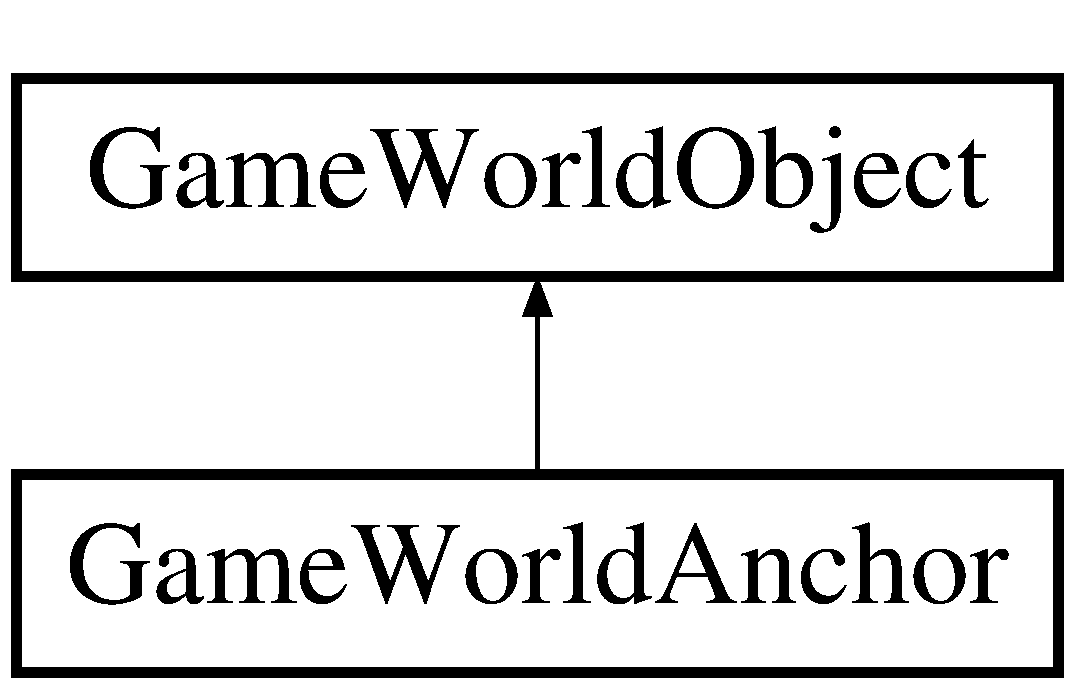
\includegraphics[height=2.000000cm]{class_game_world_anchor}
\end{center}
\end{figure}
\subsection*{Public Member Functions}
\begin{DoxyCompactItemize}
\item 
\hyperlink{class_game_world_anchor_a9b0a0ee5f92e6fabee6f6e5adc7001a2}{Game\+World\+Anchor} ()
\begin{DoxyCompactList}\small\item\em Initializes a new instance of the \hyperlink{class_game_world_anchor}{Game\+World\+Anchor} class with no \hyperlink{class_game_region}{Game\+Region} at location 0,0. \end{DoxyCompactList}\item 
\hyperlink{class_game_world_anchor_a65f7f152f39e2bbe2e76e6c7fffaeb93}{Game\+World\+Anchor} (\hyperlink{class_game_region}{Game\+Region} $\ast$anchored\+Region)
\begin{DoxyCompactList}\small\item\em Initializes a new instance of the \hyperlink{class_game_world_anchor}{Game\+World\+Anchor} class at location 0,0. \end{DoxyCompactList}\item 
\hyperlink{class_game_world_anchor_a0c6a75a46de880453962859d3d15e56e}{Game\+World\+Anchor} (\hyperlink{class_game_region}{Game\+Region} $\ast$anchored\+Region, double gx, double gy)
\begin{DoxyCompactList}\small\item\em Initializes a new instance of the \hyperlink{class_game_world_anchor}{Game\+World\+Anchor} class for the passed region at the passed starting location. \end{DoxyCompactList}\item 
virtual \hyperlink{class_game_world_anchor_a364eff1c23a49bbfc050c18efcacc48c}{$\sim$\+Game\+World\+Anchor} ()
\begin{DoxyCompactList}\small\item\em Finalizes an instance of the \hyperlink{class_game_world_anchor}{Game\+World\+Anchor} class. \end{DoxyCompactList}\item 
\mbox{\Hypertarget{class_game_world_anchor_a9402f4205c4bbd2c62d8f450cf59f178}\label{class_game_world_anchor_a9402f4205c4bbd2c62d8f450cf59f178}} 
void {\bfseries set\+Anchored\+Region} (\hyperlink{class_game_region}{Game\+Region} $\ast$region)
\item 
\mbox{\Hypertarget{class_game_world_anchor_a90f0218771154558ab23d613cc99c2f7}\label{class_game_world_anchor_a90f0218771154558ab23d613cc99c2f7}} 
\hyperlink{class_game_region}{Game\+Region} $\ast$ {\bfseries get\+Anchored\+Region} ()
\item 
virtual void \hyperlink{class_game_world_anchor_a35bafca13929710c6138950c7c38ec71}{g\+Move} (double x\+Offset, double y\+Offset)
\begin{DoxyCompactList}\small\item\em \textquotesingle{}Moves\textquotesingle{} the anchor my moving all drawable objects sf\+::sprite.\+x and sf\+::sprite.\+y in the opposite direction \end{DoxyCompactList}\item 
virtual void \hyperlink{class_game_world_anchor_accfec567c6edaa530ef6f5d5b5489d6b}{set\+Active} (bool active)
\begin{DoxyCompactList}\small\item\em Sets the \hyperlink{class_game_world_anchor}{Game\+World\+Anchor} active. \end{DoxyCompactList}\end{DoxyCompactItemize}
\subsection*{Protected Attributes}
\begin{DoxyCompactItemize}
\item 
\mbox{\Hypertarget{class_game_world_anchor_a3efa7371cec833e9ed49478e70b28012}\label{class_game_world_anchor_a3efa7371cec833e9ed49478e70b28012}} 
\hyperlink{class_game_region}{Game\+Region} $\ast$ {\bfseries anchored\+Region}
\end{DoxyCompactItemize}


\subsection{Detailed Description}
Anchors the center of the window to the \hyperlink{class_game_world_anchor}{Game\+World\+Anchor}. 



\subsection{Constructor \& Destructor Documentation}
\mbox{\Hypertarget{class_game_world_anchor_a9b0a0ee5f92e6fabee6f6e5adc7001a2}\label{class_game_world_anchor_a9b0a0ee5f92e6fabee6f6e5adc7001a2}} 
\index{Game\+World\+Anchor@{Game\+World\+Anchor}!Game\+World\+Anchor@{Game\+World\+Anchor}}
\index{Game\+World\+Anchor@{Game\+World\+Anchor}!Game\+World\+Anchor@{Game\+World\+Anchor}}
\subsubsection{\texorpdfstring{Game\+World\+Anchor()}{GameWorldAnchor()}\hspace{0.1cm}{\footnotesize\ttfamily [1/3]}}
{\footnotesize\ttfamily Game\+World\+Anchor\+::\+Game\+World\+Anchor (\begin{DoxyParamCaption}{ }\end{DoxyParamCaption})}



Initializes a new instance of the \hyperlink{class_game_world_anchor}{Game\+World\+Anchor} class with no \hyperlink{class_game_region}{Game\+Region} at location 0,0. 

\mbox{\Hypertarget{class_game_world_anchor_a65f7f152f39e2bbe2e76e6c7fffaeb93}\label{class_game_world_anchor_a65f7f152f39e2bbe2e76e6c7fffaeb93}} 
\index{Game\+World\+Anchor@{Game\+World\+Anchor}!Game\+World\+Anchor@{Game\+World\+Anchor}}
\index{Game\+World\+Anchor@{Game\+World\+Anchor}!Game\+World\+Anchor@{Game\+World\+Anchor}}
\subsubsection{\texorpdfstring{Game\+World\+Anchor()}{GameWorldAnchor()}\hspace{0.1cm}{\footnotesize\ttfamily [2/3]}}
{\footnotesize\ttfamily Game\+World\+Anchor\+::\+Game\+World\+Anchor (\begin{DoxyParamCaption}\item[{\hyperlink{class_game_region}{Game\+Region} $\ast$}]{anchored\+Region }\end{DoxyParamCaption})\hspace{0.3cm}{\ttfamily [explicit]}}



Initializes a new instance of the \hyperlink{class_game_world_anchor}{Game\+World\+Anchor} class at location 0,0. 


\begin{DoxyParams}{Parameters}
{\em anchored\+Region} & Region attached to this anchor. Every drawable item will be drawn relative to the anchors position. \\
\hline
\end{DoxyParams}
\mbox{\Hypertarget{class_game_world_anchor_a0c6a75a46de880453962859d3d15e56e}\label{class_game_world_anchor_a0c6a75a46de880453962859d3d15e56e}} 
\index{Game\+World\+Anchor@{Game\+World\+Anchor}!Game\+World\+Anchor@{Game\+World\+Anchor}}
\index{Game\+World\+Anchor@{Game\+World\+Anchor}!Game\+World\+Anchor@{Game\+World\+Anchor}}
\subsubsection{\texorpdfstring{Game\+World\+Anchor()}{GameWorldAnchor()}\hspace{0.1cm}{\footnotesize\ttfamily [3/3]}}
{\footnotesize\ttfamily Game\+World\+Anchor\+::\+Game\+World\+Anchor (\begin{DoxyParamCaption}\item[{\hyperlink{class_game_region}{Game\+Region} $\ast$}]{anchored\+Region,  }\item[{double}]{gx,  }\item[{double}]{gy }\end{DoxyParamCaption})}



Initializes a new instance of the \hyperlink{class_game_world_anchor}{Game\+World\+Anchor} class for the passed region at the passed starting location. 


\begin{DoxyParams}{Parameters}
{\em anchored\+Region} & The region attached to this anchor. Every drawable item will be drawn relative to the anchors position.\\
\hline
{\em gx} & The x starting position of the anchor. Used to determine the initial offset of drawable items. \\
\hline
{\em gy} & The y starting position of the anchor. Used to determine the initial offset of drawable items. \\
\hline
\end{DoxyParams}
\mbox{\Hypertarget{class_game_world_anchor_a364eff1c23a49bbfc050c18efcacc48c}\label{class_game_world_anchor_a364eff1c23a49bbfc050c18efcacc48c}} 
\index{Game\+World\+Anchor@{Game\+World\+Anchor}!````~Game\+World\+Anchor@{$\sim$\+Game\+World\+Anchor}}
\index{````~Game\+World\+Anchor@{$\sim$\+Game\+World\+Anchor}!Game\+World\+Anchor@{Game\+World\+Anchor}}
\subsubsection{\texorpdfstring{$\sim$\+Game\+World\+Anchor()}{~GameWorldAnchor()}}
{\footnotesize\ttfamily Game\+World\+Anchor\+::$\sim$\+Game\+World\+Anchor (\begin{DoxyParamCaption}{ }\end{DoxyParamCaption})\hspace{0.3cm}{\ttfamily [virtual]}}



Finalizes an instance of the \hyperlink{class_game_world_anchor}{Game\+World\+Anchor} class. 



\subsection{Member Function Documentation}
\mbox{\Hypertarget{class_game_world_anchor_a35bafca13929710c6138950c7c38ec71}\label{class_game_world_anchor_a35bafca13929710c6138950c7c38ec71}} 
\index{Game\+World\+Anchor@{Game\+World\+Anchor}!g\+Move@{g\+Move}}
\index{g\+Move@{g\+Move}!Game\+World\+Anchor@{Game\+World\+Anchor}}
\subsubsection{\texorpdfstring{g\+Move()}{gMove()}}
{\footnotesize\ttfamily void Game\+World\+Anchor\+::g\+Move (\begin{DoxyParamCaption}\item[{double}]{x\+Offset,  }\item[{double}]{y\+Offset }\end{DoxyParamCaption})\hspace{0.3cm}{\ttfamily [virtual]}}



\textquotesingle{}Moves\textquotesingle{} the anchor my moving all drawable objects sf\+::sprite.\+x and sf\+::sprite.\+y in the opposite direction 


\begin{DoxyParams}{Parameters}
{\em x\+Offset} & The x offset.\\
\hline
{\em y\+Offset} & The y offset.\\
\hline
\end{DoxyParams}


Implements \hyperlink{class_game_world_object_a3ddbcf57e6eb43cb4aaec7ac347d4e17}{Game\+World\+Object}.

\mbox{\Hypertarget{class_game_world_anchor_accfec567c6edaa530ef6f5d5b5489d6b}\label{class_game_world_anchor_accfec567c6edaa530ef6f5d5b5489d6b}} 
\index{Game\+World\+Anchor@{Game\+World\+Anchor}!set\+Active@{set\+Active}}
\index{set\+Active@{set\+Active}!Game\+World\+Anchor@{Game\+World\+Anchor}}
\subsubsection{\texorpdfstring{set\+Active()}{setActive()}}
{\footnotesize\ttfamily void Game\+World\+Anchor\+::set\+Active (\begin{DoxyParamCaption}\item[{bool}]{active }\end{DoxyParamCaption})\hspace{0.3cm}{\ttfamily [virtual]}}



Sets the \hyperlink{class_game_world_anchor}{Game\+World\+Anchor} active. 


\begin{DoxyParams}{Parameters}
{\em active} & if set to {\ttfamily true} \mbox{[}active\mbox{]}.\\
\hline
\end{DoxyParams}


Implements \hyperlink{class_game_world_object_a79d89ff68b9334b454300cf855719b77}{Game\+World\+Object}.



The documentation for this class was generated from the following files\+:\begin{DoxyCompactItemize}
\item 
E\+:/\+Programing/\+Programing/\+Cpp/\+Game\+Backbone/\+Game\+Backbone/Game\+World\+Anchor.\+h\item 
E\+:/\+Programing/\+Programing/\+Cpp/\+Game\+Backbone/\+Game\+Backbone/Game\+World\+Anchor.\+cpp\end{DoxyCompactItemize}

\hypertarget{class_game_world_animated_sprite}{}\section{Game\+World\+Animated\+Sprite Class Reference}
\label{class_game_world_animated_sprite}\index{Game\+World\+Animated\+Sprite@{Game\+World\+Animated\+Sprite}}


An \hyperlink{class_animated_sprite}{Animated\+Sprite} that exists in a game world and tracks its position within the game world.  




{\ttfamily \#include $<$Game\+World\+Animated\+Sprite.\+h$>$}

Inheritance diagram for Game\+World\+Animated\+Sprite\+:\begin{figure}[H]
\begin{center}
\leavevmode
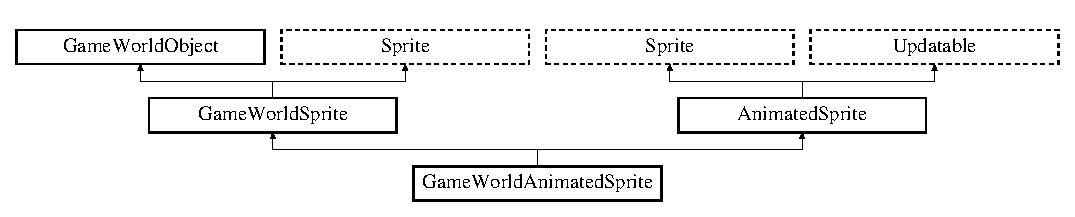
\includegraphics[height=2.470588cm]{class_game_world_animated_sprite}
\end{center}
\end{figure}
\subsection*{Public Member Functions}
\begin{DoxyCompactItemize}
\item 
\hyperlink{class_game_world_animated_sprite_a3833958136cf7e0f4a0141006e48e598}{Game\+World\+Animated\+Sprite} ()
\begin{DoxyCompactList}\small\item\em Initializes a new instance of the \hyperlink{class_game_world_animated_sprite}{Game\+World\+Animated\+Sprite} class. No texture or animations are assigned. \end{DoxyCompactList}\item 
\hyperlink{class_game_world_animated_sprite_a6b80254cbd23ab70708c9a48fbc33ce7}{Game\+World\+Animated\+Sprite} (const sf\+::\+Texture \&texture)
\begin{DoxyCompactList}\small\item\em Initializes a new instance of the \hyperlink{class_game_world_animated_sprite}{Game\+World\+Animated\+Sprite} class. The \hyperlink{class_game_world_animated_sprite}{Game\+World\+Animated\+Sprite} is given a texture, but is given no animations. \end{DoxyCompactList}\item 
\hyperlink{class_game_world_animated_sprite_af8277765bcbb4eb8b5621c6141324b94}{Game\+World\+Animated\+Sprite} (const sf\+::\+Texture \&texture, \hyperlink{class_animation_set}{Animation\+Set} $\ast$animations)
\begin{DoxyCompactList}\small\item\em Initializes a new instance of the \hyperlink{class_game_world_animated_sprite}{Game\+World\+Animated\+Sprite} class. The \hyperlink{class_game_world_animated_sprite}{Game\+World\+Animated\+Sprite} is given a texture, and assigned animations. The first frame of the first animation is set to active. \end{DoxyCompactList}\item 
virtual \hyperlink{class_game_world_animated_sprite_a33868dd12e9d7496e47760a765b55d87}{$\sim$\+Game\+World\+Animated\+Sprite} ()
\begin{DoxyCompactList}\small\item\em Finalizes an instance of the \hyperlink{class_game_world_animated_sprite}{Game\+World\+Animated\+Sprite} class. \end{DoxyCompactList}\item 
virtual void \hyperlink{class_game_world_animated_sprite_ac1aa0ef5ec1a3278934238ea214624a4}{g\+Move} (double x\+Offset, double y\+Offset)
\begin{DoxyCompactList}\small\item\em Changes the position of the sprite in the game world by the given offsets \end{DoxyCompactList}\item 
virtual void \hyperlink{class_game_world_animated_sprite_a625b0d3876fbac51995bf048e94fd7e5}{set\+Active} (bool active)
\begin{DoxyCompactList}\small\item\em Sets the \hyperlink{class_game_world_animated_sprite}{Game\+World\+Animated\+Sprite} active. \end{DoxyCompactList}\item 
virtual void \hyperlink{class_game_world_animated_sprite_a6fab62c5ed11541027a88c695a8b6147}{update} (sf\+::\+Time current\+Time)
\begin{DoxyCompactList}\small\item\em Moves the next frame of the active animation if the sprite is animating. \end{DoxyCompactList}\end{DoxyCompactItemize}
\subsection*{Additional Inherited Members}


\subsection{Detailed Description}
An \hyperlink{class_animated_sprite}{Animated\+Sprite} that exists in a game world and tracks its position within the game world. 



\subsection{Constructor \& Destructor Documentation}
\mbox{\Hypertarget{class_game_world_animated_sprite_a3833958136cf7e0f4a0141006e48e598}\label{class_game_world_animated_sprite_a3833958136cf7e0f4a0141006e48e598}} 
\index{Game\+World\+Animated\+Sprite@{Game\+World\+Animated\+Sprite}!Game\+World\+Animated\+Sprite@{Game\+World\+Animated\+Sprite}}
\index{Game\+World\+Animated\+Sprite@{Game\+World\+Animated\+Sprite}!Game\+World\+Animated\+Sprite@{Game\+World\+Animated\+Sprite}}
\subsubsection{\texorpdfstring{Game\+World\+Animated\+Sprite()}{GameWorldAnimatedSprite()}\hspace{0.1cm}{\footnotesize\ttfamily [1/3]}}
{\footnotesize\ttfamily Game\+World\+Animated\+Sprite\+::\+Game\+World\+Animated\+Sprite (\begin{DoxyParamCaption}{ }\end{DoxyParamCaption})}



Initializes a new instance of the \hyperlink{class_game_world_animated_sprite}{Game\+World\+Animated\+Sprite} class. No texture or animations are assigned. 

\mbox{\Hypertarget{class_game_world_animated_sprite_a6b80254cbd23ab70708c9a48fbc33ce7}\label{class_game_world_animated_sprite_a6b80254cbd23ab70708c9a48fbc33ce7}} 
\index{Game\+World\+Animated\+Sprite@{Game\+World\+Animated\+Sprite}!Game\+World\+Animated\+Sprite@{Game\+World\+Animated\+Sprite}}
\index{Game\+World\+Animated\+Sprite@{Game\+World\+Animated\+Sprite}!Game\+World\+Animated\+Sprite@{Game\+World\+Animated\+Sprite}}
\subsubsection{\texorpdfstring{Game\+World\+Animated\+Sprite()}{GameWorldAnimatedSprite()}\hspace{0.1cm}{\footnotesize\ttfamily [2/3]}}
{\footnotesize\ttfamily Game\+World\+Animated\+Sprite\+::\+Game\+World\+Animated\+Sprite (\begin{DoxyParamCaption}\item[{const sf\+::\+Texture \&}]{texture }\end{DoxyParamCaption})\hspace{0.3cm}{\ttfamily [explicit]}}



Initializes a new instance of the \hyperlink{class_game_world_animated_sprite}{Game\+World\+Animated\+Sprite} class. The \hyperlink{class_game_world_animated_sprite}{Game\+World\+Animated\+Sprite} is given a texture, but is given no animations. 


\begin{DoxyParams}{Parameters}
{\em texture} & The texture.\\
\hline
\end{DoxyParams}
\mbox{\Hypertarget{class_game_world_animated_sprite_af8277765bcbb4eb8b5621c6141324b94}\label{class_game_world_animated_sprite_af8277765bcbb4eb8b5621c6141324b94}} 
\index{Game\+World\+Animated\+Sprite@{Game\+World\+Animated\+Sprite}!Game\+World\+Animated\+Sprite@{Game\+World\+Animated\+Sprite}}
\index{Game\+World\+Animated\+Sprite@{Game\+World\+Animated\+Sprite}!Game\+World\+Animated\+Sprite@{Game\+World\+Animated\+Sprite}}
\subsubsection{\texorpdfstring{Game\+World\+Animated\+Sprite()}{GameWorldAnimatedSprite()}\hspace{0.1cm}{\footnotesize\ttfamily [3/3]}}
{\footnotesize\ttfamily Game\+World\+Animated\+Sprite\+::\+Game\+World\+Animated\+Sprite (\begin{DoxyParamCaption}\item[{const sf\+::\+Texture \&}]{texture,  }\item[{\hyperlink{class_animation_set}{Animation\+Set} $\ast$}]{animations }\end{DoxyParamCaption})}



Initializes a new instance of the \hyperlink{class_game_world_animated_sprite}{Game\+World\+Animated\+Sprite} class. The \hyperlink{class_game_world_animated_sprite}{Game\+World\+Animated\+Sprite} is given a texture, and assigned animations. The first frame of the first animation is set to active. 


\begin{DoxyParams}{Parameters}
{\em texture} & The texture.\\
\hline
{\em animations} & The animations.\\
\hline
\end{DoxyParams}
\mbox{\Hypertarget{class_game_world_animated_sprite_a33868dd12e9d7496e47760a765b55d87}\label{class_game_world_animated_sprite_a33868dd12e9d7496e47760a765b55d87}} 
\index{Game\+World\+Animated\+Sprite@{Game\+World\+Animated\+Sprite}!````~Game\+World\+Animated\+Sprite@{$\sim$\+Game\+World\+Animated\+Sprite}}
\index{````~Game\+World\+Animated\+Sprite@{$\sim$\+Game\+World\+Animated\+Sprite}!Game\+World\+Animated\+Sprite@{Game\+World\+Animated\+Sprite}}
\subsubsection{\texorpdfstring{$\sim$\+Game\+World\+Animated\+Sprite()}{~GameWorldAnimatedSprite()}}
{\footnotesize\ttfamily Game\+World\+Animated\+Sprite\+::$\sim$\+Game\+World\+Animated\+Sprite (\begin{DoxyParamCaption}{ }\end{DoxyParamCaption})\hspace{0.3cm}{\ttfamily [virtual]}}



Finalizes an instance of the \hyperlink{class_game_world_animated_sprite}{Game\+World\+Animated\+Sprite} class. 



\subsection{Member Function Documentation}
\mbox{\Hypertarget{class_game_world_animated_sprite_ac1aa0ef5ec1a3278934238ea214624a4}\label{class_game_world_animated_sprite_ac1aa0ef5ec1a3278934238ea214624a4}} 
\index{Game\+World\+Animated\+Sprite@{Game\+World\+Animated\+Sprite}!g\+Move@{g\+Move}}
\index{g\+Move@{g\+Move}!Game\+World\+Animated\+Sprite@{Game\+World\+Animated\+Sprite}}
\subsubsection{\texorpdfstring{g\+Move()}{gMove()}}
{\footnotesize\ttfamily void Game\+World\+Animated\+Sprite\+::g\+Move (\begin{DoxyParamCaption}\item[{double}]{x\+Offset,  }\item[{double}]{y\+Offset }\end{DoxyParamCaption})\hspace{0.3cm}{\ttfamily [virtual]}}



Changes the position of the sprite in the game world by the given offsets 


\begin{DoxyParams}{Parameters}
{\em x\+Offset} & The x offset.\\
\hline
{\em y\+Offset} & The y offset.\\
\hline
\end{DoxyParams}


Reimplemented from \hyperlink{class_game_world_sprite_ad2374a50582a6eb9e4da3cd2115dad08}{Game\+World\+Sprite}.

\mbox{\Hypertarget{class_game_world_animated_sprite_a625b0d3876fbac51995bf048e94fd7e5}\label{class_game_world_animated_sprite_a625b0d3876fbac51995bf048e94fd7e5}} 
\index{Game\+World\+Animated\+Sprite@{Game\+World\+Animated\+Sprite}!set\+Active@{set\+Active}}
\index{set\+Active@{set\+Active}!Game\+World\+Animated\+Sprite@{Game\+World\+Animated\+Sprite}}
\subsubsection{\texorpdfstring{set\+Active()}{setActive()}}
{\footnotesize\ttfamily void Game\+World\+Animated\+Sprite\+::set\+Active (\begin{DoxyParamCaption}\item[{bool}]{active }\end{DoxyParamCaption})\hspace{0.3cm}{\ttfamily [virtual]}}



Sets the \hyperlink{class_game_world_animated_sprite}{Game\+World\+Animated\+Sprite} active. 


\begin{DoxyParams}{Parameters}
{\em active} & if set to {\ttfamily true} \mbox{[}active\mbox{]}.\\
\hline
\end{DoxyParams}


Reimplemented from \hyperlink{class_game_world_sprite_a4b8597b947076f847d20c66be7db8847}{Game\+World\+Sprite}.

\mbox{\Hypertarget{class_game_world_animated_sprite_a6fab62c5ed11541027a88c695a8b6147}\label{class_game_world_animated_sprite_a6fab62c5ed11541027a88c695a8b6147}} 
\index{Game\+World\+Animated\+Sprite@{Game\+World\+Animated\+Sprite}!update@{update}}
\index{update@{update}!Game\+World\+Animated\+Sprite@{Game\+World\+Animated\+Sprite}}
\subsubsection{\texorpdfstring{update()}{update()}}
{\footnotesize\ttfamily void Game\+World\+Animated\+Sprite\+::update (\begin{DoxyParamCaption}\item[{sf\+::\+Time}]{current\+Time }\end{DoxyParamCaption})\hspace{0.3cm}{\ttfamily [virtual]}}



Moves the next frame of the active animation if the sprite is animating. 


\begin{DoxyParams}{Parameters}
{\em current\+Time} & The current time.\\
\hline
\end{DoxyParams}


Reimplemented from \hyperlink{class_animated_sprite_afdeda3e3030963a8ba290e23e48acc40}{Animated\+Sprite}.



The documentation for this class was generated from the following files\+:\begin{DoxyCompactItemize}
\item 
E\+:/\+Programing/\+Programing/\+Cpp/\+Game\+Backbone/\+Game\+Backbone/Game\+World\+Animated\+Sprite.\+h\item 
E\+:/\+Programing/\+Programing/\+Cpp/\+Game\+Backbone/\+Game\+Backbone/Game\+World\+Animated\+Sprite.\+cpp\end{DoxyCompactItemize}

\hypertarget{class_game_world_compound_sprite2}{}\section{Game\+World\+Compound\+Sprite2 Class Reference}
\label{class_game_world_compound_sprite2}\index{Game\+World\+Compound\+Sprite2@{Game\+World\+Compound\+Sprite2}}


A \hyperlink{class_compound_sprite}{Compound\+Sprite} that exists withing a game world and tracks its position withing the game world.  




{\ttfamily \#include $<$Game\+World\+Compound\+Sprite2.\+h$>$}

Inheritance diagram for Game\+World\+Compound\+Sprite2\+:\begin{figure}[H]
\begin{center}
\leavevmode
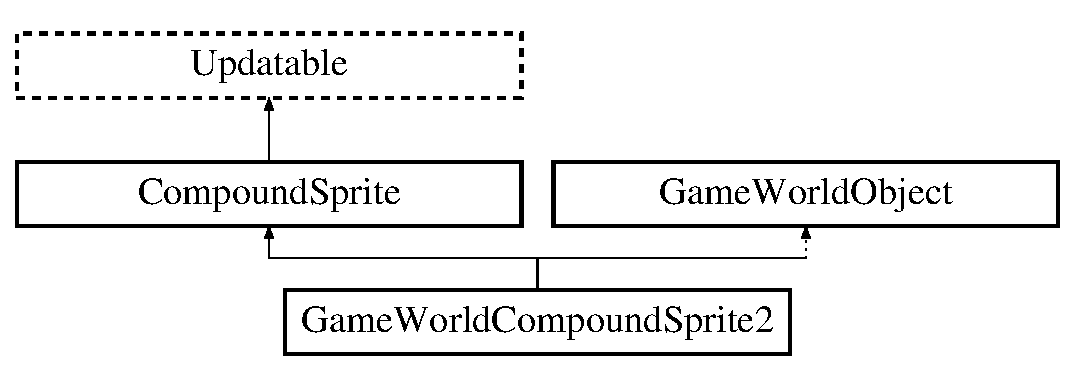
\includegraphics[height=3.000000cm]{class_game_world_compound_sprite2}
\end{center}
\end{figure}
\subsection*{Public Member Functions}
\begin{DoxyCompactItemize}
\item 
\hyperlink{class_game_world_compound_sprite2_a09c16ebe74d35c5d56259ec8b1f6c8ca}{Game\+World\+Compound\+Sprite2} (const std\+::vector$<$ sf\+::\+Sprite $\ast$$>$ \&sprites, const std\+::vector$<$ \hyperlink{class_animated_sprite}{Animated\+Sprite} $\ast$$>$ \&animated\+Sprites)
\begin{DoxyCompactList}\small\item\em Initializes a new instance of the \hyperlink{class_game_world_compound_sprite2}{Game\+World\+Compound\+Sprite2} class. Stores the passed groups of sf\+::\+Sprite and \hyperlink{class_animated_sprite}{Animated\+Sprite} as components of the \hyperlink{class_compound_sprite}{Compound\+Sprite}. \end{DoxyCompactList}\item 
virtual \hyperlink{class_game_world_compound_sprite2_ab1a2a138336d0046521df6693cf88db5}{$\sim$\+Game\+World\+Compound\+Sprite2} ()
\begin{DoxyCompactList}\small\item\em Finalizes an instance of the \hyperlink{class_game_world_compound_sprite2}{Game\+World\+Compound\+Sprite2} class. \end{DoxyCompactList}\item 
virtual void \hyperlink{class_game_world_compound_sprite2_a068bdce311f91566550409016df88489}{update} (sf\+::\+Time current\+Time)
\begin{DoxyCompactList}\small\item\em Updates each animated sprite in the \hyperlink{class_game_world_compound_sprite2}{Game\+World\+Compound\+Sprite2}. \end{DoxyCompactList}\item 
virtual void \hyperlink{class_game_world_compound_sprite2_aa45dc19c6010d86e90832f129dd1e327}{g\+Move} (double x\+Offset, double y\+Offset)
\begin{DoxyCompactList}\small\item\em Changes the position of the \hyperlink{class_game_world_compound_sprite2}{Game\+World\+Compound\+Sprite2} in the game world by the given offsets. \end{DoxyCompactList}\item 
virtual void \hyperlink{class_game_world_compound_sprite2_a773426feff97b69af22941f84a7ee40c}{set\+Active} (bool active)
\begin{DoxyCompactList}\small\item\em Sets the \hyperlink{class_game_world_compound_sprite2}{Game\+World\+Compound\+Sprite2} active. \end{DoxyCompactList}\end{DoxyCompactItemize}
\subsection*{Additional Inherited Members}


\subsection{Detailed Description}
A \hyperlink{class_compound_sprite}{Compound\+Sprite} that exists withing a game world and tracks its position withing the game world. 



\subsection{Constructor \& Destructor Documentation}
\mbox{\Hypertarget{class_game_world_compound_sprite2_a09c16ebe74d35c5d56259ec8b1f6c8ca}\label{class_game_world_compound_sprite2_a09c16ebe74d35c5d56259ec8b1f6c8ca}} 
\index{Game\+World\+Compound\+Sprite2@{Game\+World\+Compound\+Sprite2}!Game\+World\+Compound\+Sprite2@{Game\+World\+Compound\+Sprite2}}
\index{Game\+World\+Compound\+Sprite2@{Game\+World\+Compound\+Sprite2}!Game\+World\+Compound\+Sprite2@{Game\+World\+Compound\+Sprite2}}
\subsubsection{\texorpdfstring{Game\+World\+Compound\+Sprite2()}{GameWorldCompoundSprite2()}}
{\footnotesize\ttfamily Game\+World\+Compound\+Sprite2\+::\+Game\+World\+Compound\+Sprite2 (\begin{DoxyParamCaption}\item[{const std\+::vector$<$ sf\+::\+Sprite $\ast$$>$ \&}]{sprites,  }\item[{const std\+::vector$<$ \hyperlink{class_animated_sprite}{Animated\+Sprite} $\ast$$>$ \&}]{animated\+Sprites }\end{DoxyParamCaption})}



Initializes a new instance of the \hyperlink{class_game_world_compound_sprite2}{Game\+World\+Compound\+Sprite2} class. Stores the passed groups of sf\+::\+Sprite and \hyperlink{class_animated_sprite}{Animated\+Sprite} as components of the \hyperlink{class_compound_sprite}{Compound\+Sprite}. 


\begin{DoxyParams}{Parameters}
{\em sprites} & Sprite components of the new \hyperlink{class_compound_sprite}{Compound\+Sprite}.\\
\hline
{\em animated\+Sprites} & \hyperlink{class_animated_sprite}{Animated\+Sprite} components of the new \hyperlink{class_compound_sprite}{Compound\+Sprite}\\
\hline
\end{DoxyParams}
\mbox{\Hypertarget{class_game_world_compound_sprite2_ab1a2a138336d0046521df6693cf88db5}\label{class_game_world_compound_sprite2_ab1a2a138336d0046521df6693cf88db5}} 
\index{Game\+World\+Compound\+Sprite2@{Game\+World\+Compound\+Sprite2}!````~Game\+World\+Compound\+Sprite2@{$\sim$\+Game\+World\+Compound\+Sprite2}}
\index{````~Game\+World\+Compound\+Sprite2@{$\sim$\+Game\+World\+Compound\+Sprite2}!Game\+World\+Compound\+Sprite2@{Game\+World\+Compound\+Sprite2}}
\subsubsection{\texorpdfstring{$\sim$\+Game\+World\+Compound\+Sprite2()}{~GameWorldCompoundSprite2()}}
{\footnotesize\ttfamily Game\+World\+Compound\+Sprite2\+::$\sim$\+Game\+World\+Compound\+Sprite2 (\begin{DoxyParamCaption}{ }\end{DoxyParamCaption})\hspace{0.3cm}{\ttfamily [virtual]}}



Finalizes an instance of the \hyperlink{class_game_world_compound_sprite2}{Game\+World\+Compound\+Sprite2} class. 



\subsection{Member Function Documentation}
\mbox{\Hypertarget{class_game_world_compound_sprite2_aa45dc19c6010d86e90832f129dd1e327}\label{class_game_world_compound_sprite2_aa45dc19c6010d86e90832f129dd1e327}} 
\index{Game\+World\+Compound\+Sprite2@{Game\+World\+Compound\+Sprite2}!g\+Move@{g\+Move}}
\index{g\+Move@{g\+Move}!Game\+World\+Compound\+Sprite2@{Game\+World\+Compound\+Sprite2}}
\subsubsection{\texorpdfstring{g\+Move()}{gMove()}}
{\footnotesize\ttfamily void Game\+World\+Compound\+Sprite2\+::g\+Move (\begin{DoxyParamCaption}\item[{double}]{x\+Offset,  }\item[{double}]{y\+Offset }\end{DoxyParamCaption})\hspace{0.3cm}{\ttfamily [virtual]}}



Changes the position of the \hyperlink{class_game_world_compound_sprite2}{Game\+World\+Compound\+Sprite2} in the game world by the given offsets. 


\begin{DoxyParams}{Parameters}
{\em x\+Offset} & X offset of the new position.\\
\hline
{\em y\+Offset} & Y offset of the new position.\\
\hline
\end{DoxyParams}


Implements \hyperlink{class_game_world_object_a3ddbcf57e6eb43cb4aaec7ac347d4e17}{Game\+World\+Object}.

\mbox{\Hypertarget{class_game_world_compound_sprite2_a773426feff97b69af22941f84a7ee40c}\label{class_game_world_compound_sprite2_a773426feff97b69af22941f84a7ee40c}} 
\index{Game\+World\+Compound\+Sprite2@{Game\+World\+Compound\+Sprite2}!set\+Active@{set\+Active}}
\index{set\+Active@{set\+Active}!Game\+World\+Compound\+Sprite2@{Game\+World\+Compound\+Sprite2}}
\subsubsection{\texorpdfstring{set\+Active()}{setActive()}}
{\footnotesize\ttfamily void Game\+World\+Compound\+Sprite2\+::set\+Active (\begin{DoxyParamCaption}\item[{bool}]{active }\end{DoxyParamCaption})\hspace{0.3cm}{\ttfamily [virtual]}}



Sets the \hyperlink{class_game_world_compound_sprite2}{Game\+World\+Compound\+Sprite2} active. 


\begin{DoxyParams}{Parameters}
{\em active} & if set to {\ttfamily true} \mbox{[}active\mbox{]}.\\
\hline
\end{DoxyParams}


Implements \hyperlink{class_game_world_object_a79d89ff68b9334b454300cf855719b77}{Game\+World\+Object}.

\mbox{\Hypertarget{class_game_world_compound_sprite2_a068bdce311f91566550409016df88489}\label{class_game_world_compound_sprite2_a068bdce311f91566550409016df88489}} 
\index{Game\+World\+Compound\+Sprite2@{Game\+World\+Compound\+Sprite2}!update@{update}}
\index{update@{update}!Game\+World\+Compound\+Sprite2@{Game\+World\+Compound\+Sprite2}}
\subsubsection{\texorpdfstring{update()}{update()}}
{\footnotesize\ttfamily void Game\+World\+Compound\+Sprite2\+::update (\begin{DoxyParamCaption}\item[{sf\+::\+Time}]{current\+Time }\end{DoxyParamCaption})\hspace{0.3cm}{\ttfamily [virtual]}}



Updates each animated sprite in the \hyperlink{class_game_world_compound_sprite2}{Game\+World\+Compound\+Sprite2}. 


\begin{DoxyParams}{Parameters}
{\em current\+Time} & The current time.\\
\hline
\end{DoxyParams}


Reimplemented from \hyperlink{class_compound_sprite_a0761cc2bdded00f203db7e4c6d02aa6c}{Compound\+Sprite}.



The documentation for this class was generated from the following files\+:\begin{DoxyCompactItemize}
\item 
E\+:/\+Programing/\+Programing/\+Cpp/\+Game\+Backbone/\+Game\+Backbone/Game\+World\+Compound\+Sprite2.\+h\item 
E\+:/\+Programing/\+Programing/\+Cpp/\+Game\+Backbone/\+Game\+Backbone/Game\+World\+Compound\+Sprite2.\+cpp\end{DoxyCompactItemize}

\hypertarget{class_game_world_object}{}\section{Game\+World\+Object Class Reference}
\label{class_game_world_object}\index{Game\+World\+Object@{Game\+World\+Object}}


Abstract object in the game world that keep track of its position within the game world  




{\ttfamily \#include $<$Game\+World\+Object.\+h$>$}

Inheritance diagram for Game\+World\+Object\+:\begin{figure}[H]
\begin{center}
\leavevmode
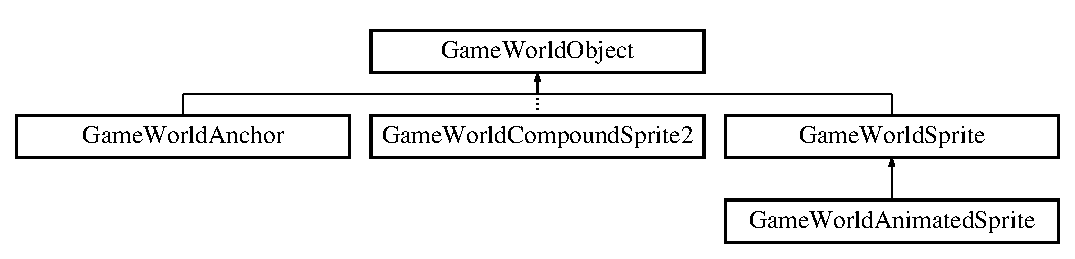
\includegraphics[height=3.000000cm]{class_game_world_object}
\end{center}
\end{figure}
\subsection*{Public Member Functions}
\begin{DoxyCompactItemize}
\item 
\hyperlink{class_game_world_object_a1c273875f7dd21cb8ec9f03b6ff26a18}{Game\+World\+Object} ()
\begin{DoxyCompactList}\small\item\em Initializes a new instance of the \hyperlink{class_game_world_compound_sprite2}{Game\+World\+Compound\+Sprite2} class. The game world position defaults to 0,0. \end{DoxyCompactList}\item 
virtual \hyperlink{class_game_world_object_aa0a604119a1f66b3a299e8a192c4b554}{$\sim$\+Game\+World\+Object} ()
\begin{DoxyCompactList}\small\item\em Finalizes an instance of the \hyperlink{class_game_world_object}{Game\+World\+Object} class. \end{DoxyCompactList}\item 
virtual void \hyperlink{class_game_world_object_a79d89ff68b9334b454300cf855719b77}{set\+Active} (bool active)=0
\begin{DoxyCompactList}\small\item\em Whether or not the \hyperlink{class_game_world_object}{Game\+World\+Object} is active in the game world\end{DoxyCompactList}\item 
double \hyperlink{class_game_world_object_a292eb95c0bb79fdceb72c35591bb1c88}{get\+Gx} ()
\begin{DoxyCompactList}\small\item\em The x position of the object in the game world. \end{DoxyCompactList}\item 
double \hyperlink{class_game_world_object_a2bfa46580715a74de892201b8043d2d2}{get\+Gy} ()
\begin{DoxyCompactList}\small\item\em Sets the y position of the object in the game world. \end{DoxyCompactList}\item 
double \hyperlink{class_game_world_object_a2c44a748bb3070545761d7e7c22c7f99}{is\+Active} ()
\begin{DoxyCompactList}\small\item\em Whether or not the \hyperlink{class_game_world_object}{Game\+World\+Object} is active in the game world. \end{DoxyCompactList}\item 
virtual void \hyperlink{class_game_world_object_a3ddbcf57e6eb43cb4aaec7ac347d4e17}{g\+Move} (double x\+Offset, double y\+Offset)=0
\begin{DoxyCompactList}\small\item\em Changes the position of the sprite in the game world by the given offsets\end{DoxyCompactList}\end{DoxyCompactItemize}
\subsection*{Protected Attributes}
\begin{DoxyCompactItemize}
\item 
\mbox{\Hypertarget{class_game_world_object_a87f4cffe1c02cef24305adade2a89dd2}\label{class_game_world_object_a87f4cffe1c02cef24305adade2a89dd2}} 
\hyperlink{struct_point2_d}{Point2D} {\bfseries gw\+Position}
\item 
\mbox{\Hypertarget{class_game_world_object_a51ccb433f7e6ed99e280840bb611596d}\label{class_game_world_object_a51ccb433f7e6ed99e280840bb611596d}} 
bool {\bfseries active}
\end{DoxyCompactItemize}


\subsection{Detailed Description}
Abstract object in the game world that keep track of its position within the game world 



\subsection{Constructor \& Destructor Documentation}
\mbox{\Hypertarget{class_game_world_object_a1c273875f7dd21cb8ec9f03b6ff26a18}\label{class_game_world_object_a1c273875f7dd21cb8ec9f03b6ff26a18}} 
\index{Game\+World\+Object@{Game\+World\+Object}!Game\+World\+Object@{Game\+World\+Object}}
\index{Game\+World\+Object@{Game\+World\+Object}!Game\+World\+Object@{Game\+World\+Object}}
\subsubsection{\texorpdfstring{Game\+World\+Object()}{GameWorldObject()}}
{\footnotesize\ttfamily Game\+World\+Object\+::\+Game\+World\+Object (\begin{DoxyParamCaption}{ }\end{DoxyParamCaption})}



Initializes a new instance of the \hyperlink{class_game_world_compound_sprite2}{Game\+World\+Compound\+Sprite2} class. The game world position defaults to 0,0. 

\mbox{\Hypertarget{class_game_world_object_aa0a604119a1f66b3a299e8a192c4b554}\label{class_game_world_object_aa0a604119a1f66b3a299e8a192c4b554}} 
\index{Game\+World\+Object@{Game\+World\+Object}!````~Game\+World\+Object@{$\sim$\+Game\+World\+Object}}
\index{````~Game\+World\+Object@{$\sim$\+Game\+World\+Object}!Game\+World\+Object@{Game\+World\+Object}}
\subsubsection{\texorpdfstring{$\sim$\+Game\+World\+Object()}{~GameWorldObject()}}
{\footnotesize\ttfamily Game\+World\+Object\+::$\sim$\+Game\+World\+Object (\begin{DoxyParamCaption}{ }\end{DoxyParamCaption})\hspace{0.3cm}{\ttfamily [virtual]}}



Finalizes an instance of the \hyperlink{class_game_world_object}{Game\+World\+Object} class. 



\subsection{Member Function Documentation}
\mbox{\Hypertarget{class_game_world_object_a292eb95c0bb79fdceb72c35591bb1c88}\label{class_game_world_object_a292eb95c0bb79fdceb72c35591bb1c88}} 
\index{Game\+World\+Object@{Game\+World\+Object}!get\+Gx@{get\+Gx}}
\index{get\+Gx@{get\+Gx}!Game\+World\+Object@{Game\+World\+Object}}
\subsubsection{\texorpdfstring{get\+Gx()}{getGx()}}
{\footnotesize\ttfamily double Game\+World\+Object\+::get\+Gx (\begin{DoxyParamCaption}{ }\end{DoxyParamCaption})}



The x position of the object in the game world. 

\begin{DoxyReturn}{Returns}

\end{DoxyReturn}
\mbox{\Hypertarget{class_game_world_object_a2bfa46580715a74de892201b8043d2d2}\label{class_game_world_object_a2bfa46580715a74de892201b8043d2d2}} 
\index{Game\+World\+Object@{Game\+World\+Object}!get\+Gy@{get\+Gy}}
\index{get\+Gy@{get\+Gy}!Game\+World\+Object@{Game\+World\+Object}}
\subsubsection{\texorpdfstring{get\+Gy()}{getGy()}}
{\footnotesize\ttfamily double Game\+World\+Object\+::get\+Gy (\begin{DoxyParamCaption}{ }\end{DoxyParamCaption})}



Sets the y position of the object in the game world. 

\begin{DoxyReturn}{Returns}

\end{DoxyReturn}
\mbox{\Hypertarget{class_game_world_object_a3ddbcf57e6eb43cb4aaec7ac347d4e17}\label{class_game_world_object_a3ddbcf57e6eb43cb4aaec7ac347d4e17}} 
\index{Game\+World\+Object@{Game\+World\+Object}!g\+Move@{g\+Move}}
\index{g\+Move@{g\+Move}!Game\+World\+Object@{Game\+World\+Object}}
\subsubsection{\texorpdfstring{g\+Move()}{gMove()}}
{\footnotesize\ttfamily virtual void Game\+World\+Object\+::g\+Move (\begin{DoxyParamCaption}\item[{double}]{x\+Offset,  }\item[{double}]{y\+Offset }\end{DoxyParamCaption})\hspace{0.3cm}{\ttfamily [pure virtual]}}



Changes the position of the sprite in the game world by the given offsets



Implemented in \hyperlink{class_game_world_anchor_a35bafca13929710c6138950c7c38ec71}{Game\+World\+Anchor}, \hyperlink{class_game_world_compound_sprite2_aa45dc19c6010d86e90832f129dd1e327}{Game\+World\+Compound\+Sprite2}, \hyperlink{class_game_world_animated_sprite_ac1aa0ef5ec1a3278934238ea214624a4}{Game\+World\+Animated\+Sprite}, and \hyperlink{class_game_world_sprite_ad2374a50582a6eb9e4da3cd2115dad08}{Game\+World\+Sprite}.

\mbox{\Hypertarget{class_game_world_object_a2c44a748bb3070545761d7e7c22c7f99}\label{class_game_world_object_a2c44a748bb3070545761d7e7c22c7f99}} 
\index{Game\+World\+Object@{Game\+World\+Object}!is\+Active@{is\+Active}}
\index{is\+Active@{is\+Active}!Game\+World\+Object@{Game\+World\+Object}}
\subsubsection{\texorpdfstring{is\+Active()}{isActive()}}
{\footnotesize\ttfamily double Game\+World\+Object\+::is\+Active (\begin{DoxyParamCaption}{ }\end{DoxyParamCaption})}



Whether or not the \hyperlink{class_game_world_object}{Game\+World\+Object} is active in the game world. 

\begin{DoxyReturn}{Returns}

\end{DoxyReturn}
\mbox{\Hypertarget{class_game_world_object_a79d89ff68b9334b454300cf855719b77}\label{class_game_world_object_a79d89ff68b9334b454300cf855719b77}} 
\index{Game\+World\+Object@{Game\+World\+Object}!set\+Active@{set\+Active}}
\index{set\+Active@{set\+Active}!Game\+World\+Object@{Game\+World\+Object}}
\subsubsection{\texorpdfstring{set\+Active()}{setActive()}}
{\footnotesize\ttfamily virtual void Game\+World\+Object\+::set\+Active (\begin{DoxyParamCaption}\item[{bool}]{active }\end{DoxyParamCaption})\hspace{0.3cm}{\ttfamily [pure virtual]}}



Whether or not the \hyperlink{class_game_world_object}{Game\+World\+Object} is active in the game world



Implemented in \hyperlink{class_game_world_anchor_accfec567c6edaa530ef6f5d5b5489d6b}{Game\+World\+Anchor}, \hyperlink{class_game_world_compound_sprite2_a773426feff97b69af22941f84a7ee40c}{Game\+World\+Compound\+Sprite2}, \hyperlink{class_game_world_animated_sprite_a625b0d3876fbac51995bf048e94fd7e5}{Game\+World\+Animated\+Sprite}, and \hyperlink{class_game_world_sprite_a4b8597b947076f847d20c66be7db8847}{Game\+World\+Sprite}.



The documentation for this class was generated from the following files\+:\begin{DoxyCompactItemize}
\item 
E\+:/\+Programing/\+Programing/\+Cpp/\+Game\+Backbone/\+Game\+Backbone/Game\+World\+Object.\+h\item 
E\+:/\+Programing/\+Programing/\+Cpp/\+Game\+Backbone/\+Game\+Backbone/Game\+World\+Object.\+cpp\end{DoxyCompactItemize}

\hypertarget{class_game_world_sprite}{}\section{Game\+World\+Sprite Class Reference}
\label{class_game_world_sprite}\index{Game\+World\+Sprite@{Game\+World\+Sprite}}


A sf\+::\+Sprite that exists withing a game world and tracks its position withing the game world.  




{\ttfamily \#include $<$Game\+World\+Sprite.\+h$>$}

Inheritance diagram for Game\+World\+Sprite\+:\begin{figure}[H]
\begin{center}
\leavevmode
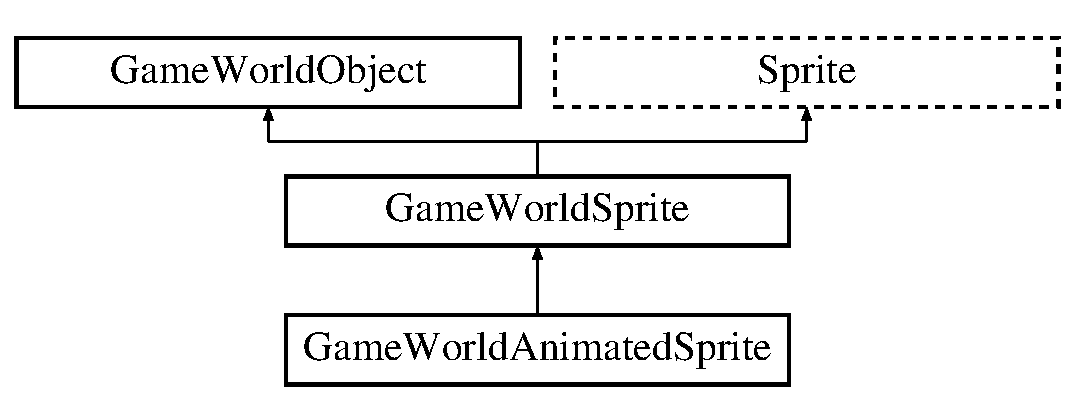
\includegraphics[height=3.000000cm]{class_game_world_sprite}
\end{center}
\end{figure}
\subsection*{Public Member Functions}
\begin{DoxyCompactItemize}
\item 
\hyperlink{class_game_world_sprite_abab91a4f2d92e1a1719a0a43d21ed62b}{Game\+World\+Sprite} ()
\begin{DoxyCompactList}\small\item\em Creates a sprite with default parameters at game world position 0,0; \end{DoxyCompactList}\item 
\hyperlink{class_game_world_sprite_a973f48586038da4f94a2b504c484918a}{Game\+World\+Sprite} (const sf\+::\+Texture \&texture)
\begin{DoxyCompactList}\small\item\em Initializes a new instance of the \hyperlink{class_game_world_sprite}{Game\+World\+Sprite} class with a default game world position of 0,0 and a valid texture \end{DoxyCompactList}\item 
\hyperlink{class_game_world_sprite_a99c58b4dfb012959edf78f66f994a6d5}{Game\+World\+Sprite} (const sf\+::\+Texture \&texture, const sf\+::\+Int\+Rect \&rectangle)
\begin{DoxyCompactList}\small\item\em Initializes a new instance of the \hyperlink{class_game_world_sprite}{Game\+World\+Sprite} class with a valid texture, a sub-\/rectangle of the source texture, default game world position of 0, 0. \end{DoxyCompactList}\item 
virtual \hyperlink{class_game_world_sprite_a2084d2b53b02071beaf7f1d81aa440f6}{$\sim$\+Game\+World\+Sprite} ()
\begin{DoxyCompactList}\small\item\em Finalizes an instance of the \hyperlink{class_game_world_sprite}{Game\+World\+Sprite} class. \end{DoxyCompactList}\item 
virtual void \hyperlink{class_game_world_sprite_ad2374a50582a6eb9e4da3cd2115dad08}{g\+Move} (double x, double y)
\begin{DoxyCompactList}\small\item\em Changes the position of the sprite in the game world by the given offsets. \end{DoxyCompactList}\item 
virtual void \hyperlink{class_game_world_sprite_a4b8597b947076f847d20c66be7db8847}{set\+Active} (bool active)
\begin{DoxyCompactList}\small\item\em Sets the \hyperlink{class_game_world_sprite}{Game\+World\+Sprite} active. \end{DoxyCompactList}\item 
virtual void \hyperlink{class_game_world_sprite_a533f3986452ad2859729d27cc09a5e53}{update} (sf\+::\+Time current\+Time)
\begin{DoxyCompactList}\small\item\em Do not use this. \end{DoxyCompactList}\end{DoxyCompactItemize}
\subsection*{Additional Inherited Members}


\subsection{Detailed Description}
A sf\+::\+Sprite that exists withing a game world and tracks its position withing the game world. 



\subsection{Constructor \& Destructor Documentation}
\mbox{\Hypertarget{class_game_world_sprite_abab91a4f2d92e1a1719a0a43d21ed62b}\label{class_game_world_sprite_abab91a4f2d92e1a1719a0a43d21ed62b}} 
\index{Game\+World\+Sprite@{Game\+World\+Sprite}!Game\+World\+Sprite@{Game\+World\+Sprite}}
\index{Game\+World\+Sprite@{Game\+World\+Sprite}!Game\+World\+Sprite@{Game\+World\+Sprite}}
\subsubsection{\texorpdfstring{Game\+World\+Sprite()}{GameWorldSprite()}\hspace{0.1cm}{\footnotesize\ttfamily [1/3]}}
{\footnotesize\ttfamily Game\+World\+Sprite\+::\+Game\+World\+Sprite (\begin{DoxyParamCaption}{ }\end{DoxyParamCaption})}



Creates a sprite with default parameters at game world position 0,0; 

\mbox{\Hypertarget{class_game_world_sprite_a973f48586038da4f94a2b504c484918a}\label{class_game_world_sprite_a973f48586038da4f94a2b504c484918a}} 
\index{Game\+World\+Sprite@{Game\+World\+Sprite}!Game\+World\+Sprite@{Game\+World\+Sprite}}
\index{Game\+World\+Sprite@{Game\+World\+Sprite}!Game\+World\+Sprite@{Game\+World\+Sprite}}
\subsubsection{\texorpdfstring{Game\+World\+Sprite()}{GameWorldSprite()}\hspace{0.1cm}{\footnotesize\ttfamily [2/3]}}
{\footnotesize\ttfamily Game\+World\+Sprite\+::\+Game\+World\+Sprite (\begin{DoxyParamCaption}\item[{const sf\+::\+Texture \&}]{texture }\end{DoxyParamCaption})\hspace{0.3cm}{\ttfamily [explicit]}}



Initializes a new instance of the \hyperlink{class_game_world_sprite}{Game\+World\+Sprite} class with a default game world position of 0,0 and a valid texture 


\begin{DoxyParams}{Parameters}
{\em texture} & The texture.\\
\hline
\end{DoxyParams}
\mbox{\Hypertarget{class_game_world_sprite_a99c58b4dfb012959edf78f66f994a6d5}\label{class_game_world_sprite_a99c58b4dfb012959edf78f66f994a6d5}} 
\index{Game\+World\+Sprite@{Game\+World\+Sprite}!Game\+World\+Sprite@{Game\+World\+Sprite}}
\index{Game\+World\+Sprite@{Game\+World\+Sprite}!Game\+World\+Sprite@{Game\+World\+Sprite}}
\subsubsection{\texorpdfstring{Game\+World\+Sprite()}{GameWorldSprite()}\hspace{0.1cm}{\footnotesize\ttfamily [3/3]}}
{\footnotesize\ttfamily Game\+World\+Sprite\+::\+Game\+World\+Sprite (\begin{DoxyParamCaption}\item[{const sf\+::\+Texture \&}]{texture,  }\item[{const sf\+::\+Int\+Rect \&}]{rectangle }\end{DoxyParamCaption})}



Initializes a new instance of the \hyperlink{class_game_world_sprite}{Game\+World\+Sprite} class with a valid texture, a sub-\/rectangle of the source texture, default game world position of 0, 0. 


\begin{DoxyParams}{Parameters}
{\em texture} & The texture.\\
\hline
{\em rectangle} & Sub-\/rectangle of the texture to assign to the sprite.\\
\hline
\end{DoxyParams}
\mbox{\Hypertarget{class_game_world_sprite_a2084d2b53b02071beaf7f1d81aa440f6}\label{class_game_world_sprite_a2084d2b53b02071beaf7f1d81aa440f6}} 
\index{Game\+World\+Sprite@{Game\+World\+Sprite}!````~Game\+World\+Sprite@{$\sim$\+Game\+World\+Sprite}}
\index{````~Game\+World\+Sprite@{$\sim$\+Game\+World\+Sprite}!Game\+World\+Sprite@{Game\+World\+Sprite}}
\subsubsection{\texorpdfstring{$\sim$\+Game\+World\+Sprite()}{~GameWorldSprite()}}
{\footnotesize\ttfamily Game\+World\+Sprite\+::$\sim$\+Game\+World\+Sprite (\begin{DoxyParamCaption}{ }\end{DoxyParamCaption})\hspace{0.3cm}{\ttfamily [virtual]}}



Finalizes an instance of the \hyperlink{class_game_world_sprite}{Game\+World\+Sprite} class. 



\subsection{Member Function Documentation}
\mbox{\Hypertarget{class_game_world_sprite_ad2374a50582a6eb9e4da3cd2115dad08}\label{class_game_world_sprite_ad2374a50582a6eb9e4da3cd2115dad08}} 
\index{Game\+World\+Sprite@{Game\+World\+Sprite}!g\+Move@{g\+Move}}
\index{g\+Move@{g\+Move}!Game\+World\+Sprite@{Game\+World\+Sprite}}
\subsubsection{\texorpdfstring{g\+Move()}{gMove()}}
{\footnotesize\ttfamily void Game\+World\+Sprite\+::g\+Move (\begin{DoxyParamCaption}\item[{double}]{x\+Offset,  }\item[{double}]{y\+Offset }\end{DoxyParamCaption})\hspace{0.3cm}{\ttfamily [virtual]}}



Changes the position of the sprite in the game world by the given offsets. 


\begin{DoxyParams}{Parameters}
{\em x\+Offset} & The x offset.\\
\hline
{\em y\+Offset} & The y offset.\\
\hline
\end{DoxyParams}


Implements \hyperlink{class_game_world_object_a3ddbcf57e6eb43cb4aaec7ac347d4e17}{Game\+World\+Object}.



Reimplemented in \hyperlink{class_game_world_animated_sprite_ac1aa0ef5ec1a3278934238ea214624a4}{Game\+World\+Animated\+Sprite}.

\mbox{\Hypertarget{class_game_world_sprite_a4b8597b947076f847d20c66be7db8847}\label{class_game_world_sprite_a4b8597b947076f847d20c66be7db8847}} 
\index{Game\+World\+Sprite@{Game\+World\+Sprite}!set\+Active@{set\+Active}}
\index{set\+Active@{set\+Active}!Game\+World\+Sprite@{Game\+World\+Sprite}}
\subsubsection{\texorpdfstring{set\+Active()}{setActive()}}
{\footnotesize\ttfamily void Game\+World\+Sprite\+::set\+Active (\begin{DoxyParamCaption}\item[{bool}]{active }\end{DoxyParamCaption})\hspace{0.3cm}{\ttfamily [virtual]}}



Sets the \hyperlink{class_game_world_sprite}{Game\+World\+Sprite} active. 


\begin{DoxyParams}{Parameters}
{\em active} & if set to {\ttfamily true} \mbox{[}active\mbox{]}.\\
\hline
\end{DoxyParams}


Implements \hyperlink{class_game_world_object_a79d89ff68b9334b454300cf855719b77}{Game\+World\+Object}.



Reimplemented in \hyperlink{class_game_world_animated_sprite_a625b0d3876fbac51995bf048e94fd7e5}{Game\+World\+Animated\+Sprite}.

\mbox{\Hypertarget{class_game_world_sprite_a533f3986452ad2859729d27cc09a5e53}\label{class_game_world_sprite_a533f3986452ad2859729d27cc09a5e53}} 
\index{Game\+World\+Sprite@{Game\+World\+Sprite}!update@{update}}
\index{update@{update}!Game\+World\+Sprite@{Game\+World\+Sprite}}
\subsubsection{\texorpdfstring{update()}{update()}}
{\footnotesize\ttfamily void Game\+World\+Sprite\+::update (\begin{DoxyParamCaption}\item[{sf\+::\+Time}]{current\+Time }\end{DoxyParamCaption})\hspace{0.3cm}{\ttfamily [virtual]}}



Do not use this. 


\begin{DoxyParams}{Parameters}
{\em current\+Time} & The current time.\\
\hline
\end{DoxyParams}


Reimplemented in \hyperlink{class_game_world_animated_sprite_a6fab62c5ed11541027a88c695a8b6147}{Game\+World\+Animated\+Sprite}.



The documentation for this class was generated from the following files\+:\begin{DoxyCompactItemize}
\item 
E\+:/\+Programing/\+Programing/\+Cpp/\+Game\+Backbone/\+Game\+Backbone/Game\+World\+Sprite.\+h\item 
E\+:/\+Programing/\+Programing/\+Cpp/\+Game\+Backbone/\+Game\+Backbone/Game\+World\+Sprite.\+cpp\end{DoxyCompactItemize}

\hypertarget{struct_navigation_hex_data}{}\section{Navigation\+Hex\+Data Struct Reference}
\label{struct_navigation_hex_data}\index{Navigation\+Hex\+Data@{Navigation\+Hex\+Data}}


Information stored in each navigation hex.  




{\ttfamily \#include $<$Navigation\+Hex\+Data.\+h$>$}

\subsection*{Public Attributes}
\begin{DoxyCompactItemize}
\item 
\mbox{\Hypertarget{struct_navigation_hex_data_aa04d0d93b848701da777f0e03920d51f}\label{struct_navigation_hex_data_aa04d0d93b848701da777f0e03920d51f}} 
int {\bfseries weight}
\item 
\mbox{\Hypertarget{struct_navigation_hex_data_a608ab4b8190230320ae175625ab9e756}\label{struct_navigation_hex_data_a608ab4b8190230320ae175625ab9e756}} 
unsigned int {\bfseries blocker\+Dist}
\end{DoxyCompactItemize}


\subsection{Detailed Description}
Information stored in each navigation hex. 



The documentation for this struct was generated from the following file\+:\begin{DoxyCompactItemize}
\item 
E\+:/\+Programing/\+Programing/\+Cpp/\+Game\+Backbone/\+Game\+Backbone/Navigation\+Hex\+Data.\+h\end{DoxyCompactItemize}

\hypertarget{class_pathfinder}{}\section{Pathfinder Class Reference}
\label{class_pathfinder}\index{Pathfinder@{Pathfinder}}


used to calculate groups of paths in one navigation grid.  




{\ttfamily \#include $<$Path\+Finder.\+h$>$}

\subsection*{Public Member Functions}
\begin{DoxyCompactItemize}
\item 
\hyperlink{class_pathfinder_af562d840858cf2b369fcee51f5069456}{Pathfinder} ()
\begin{DoxyCompactList}\small\item\em Creates a Path\+Finder with a null navigation grid. \end{DoxyCompactList}\item 
\hyperlink{class_pathfinder_ac1e4958b42424bbc9c5868cff3296e8c}{Pathfinder} (\hyperlink{class_array3_d}{Navigation\+Grid} $\ast$navigation\+Grid)
\begin{DoxyCompactList}\small\item\em Creates a Path\+Finder with an assigned navigation grid. \end{DoxyCompactList}\item 
void \hyperlink{class_pathfinder_ab2077e60f522a2d422f8b0e63cc4aa40}{set\+Navigation\+Grid} (\hyperlink{class_array3_d}{Navigation\+Grid} $\ast$navigation\+Grid)
\begin{DoxyCompactList}\small\item\em Sets the navigation grid. \end{DoxyCompactList}\item 
\hyperlink{class_array3_d}{Navigation\+Grid} $\ast$ \hyperlink{class_pathfinder_ab8d678b30e172c242923fb55f0a7a028}{get\+Navigation\+Grid} ()
\begin{DoxyCompactList}\small\item\em Gets the navigation grid. \end{DoxyCompactList}\item 
void \hyperlink{class_pathfinder_ab92e595aab257245d23dc19ff68f04fa}{path\+Find} (const std\+::vector$<$ \hyperlink{struct_path_request}{Path\+Request} $>$ \&path\+Requests, std\+::vector$<$ std\+::list$<$ sf\+::\+Vector3i $>$$>$ $\ast$const returned\+Paths)
\begin{DoxyCompactList}\small\item\em Creates an unblocked path of adjacent hexes to for each path request. \end{DoxyCompactList}\end{DoxyCompactItemize}


\subsection{Detailed Description}
used to calculate groups of paths in one navigation grid. 



\subsection{Constructor \& Destructor Documentation}
\mbox{\Hypertarget{class_pathfinder_af562d840858cf2b369fcee51f5069456}\label{class_pathfinder_af562d840858cf2b369fcee51f5069456}} 
\index{Pathfinder@{Pathfinder}!Pathfinder@{Pathfinder}}
\index{Pathfinder@{Pathfinder}!Pathfinder@{Pathfinder}}
\subsubsection{\texorpdfstring{Pathfinder()}{Pathfinder()}\hspace{0.1cm}{\footnotesize\ttfamily [1/2]}}
{\footnotesize\ttfamily Pathfinder\+::\+Pathfinder (\begin{DoxyParamCaption}{ }\end{DoxyParamCaption})}



Creates a Path\+Finder with a null navigation grid. 

\mbox{\Hypertarget{class_pathfinder_ac1e4958b42424bbc9c5868cff3296e8c}\label{class_pathfinder_ac1e4958b42424bbc9c5868cff3296e8c}} 
\index{Pathfinder@{Pathfinder}!Pathfinder@{Pathfinder}}
\index{Pathfinder@{Pathfinder}!Pathfinder@{Pathfinder}}
\subsubsection{\texorpdfstring{Pathfinder()}{Pathfinder()}\hspace{0.1cm}{\footnotesize\ttfamily [2/2]}}
{\footnotesize\ttfamily Pathfinder\+::\+Pathfinder (\begin{DoxyParamCaption}\item[{\hyperlink{class_array3_d}{Navigation\+Grid} $\ast$}]{navigation\+Grid }\end{DoxyParamCaption})\hspace{0.3cm}{\ttfamily [explicit]}}



Creates a Path\+Finder with an assigned navigation grid. 


\begin{DoxyParams}{Parameters}
{\em navigation\+Grid} & Three dimensional grid to be used when path-\/finding. \\
\hline
\end{DoxyParams}


\subsection{Member Function Documentation}
\mbox{\Hypertarget{class_pathfinder_ab8d678b30e172c242923fb55f0a7a028}\label{class_pathfinder_ab8d678b30e172c242923fb55f0a7a028}} 
\index{Pathfinder@{Pathfinder}!get\+Navigation\+Grid@{get\+Navigation\+Grid}}
\index{get\+Navigation\+Grid@{get\+Navigation\+Grid}!Pathfinder@{Pathfinder}}
\subsubsection{\texorpdfstring{get\+Navigation\+Grid()}{getNavigationGrid()}}
{\footnotesize\ttfamily \hyperlink{class_array3_d}{Navigation\+Grid} $\ast$ Pathfinder\+::get\+Navigation\+Grid (\begin{DoxyParamCaption}{ }\end{DoxyParamCaption})}



Gets the navigation grid. 

\begin{DoxyReturn}{Returns}
Navigation\+Grid pointer
\end{DoxyReturn}
\mbox{\Hypertarget{class_pathfinder_ab92e595aab257245d23dc19ff68f04fa}\label{class_pathfinder_ab92e595aab257245d23dc19ff68f04fa}} 
\index{Pathfinder@{Pathfinder}!path\+Find@{path\+Find}}
\index{path\+Find@{path\+Find}!Pathfinder@{Pathfinder}}
\subsubsection{\texorpdfstring{path\+Find()}{pathFind()}}
{\footnotesize\ttfamily void Pathfinder\+::path\+Find (\begin{DoxyParamCaption}\item[{const std\+::vector$<$ \hyperlink{struct_path_request}{Path\+Request} $>$ \&}]{path\+Requests,  }\item[{std\+::vector$<$ std\+::list$<$ sf\+::\+Vector3i $>$$>$ $\ast$const}]{returned\+Paths }\end{DoxyParamCaption})}



Creates an unblocked path of adjacent hexes to for each path request. 


\begin{DoxyParams}{Parameters}
{\em path\+Requests} & vector containing the requirements for each path.\\
\hline
{\em returned\+Paths} & vector containing the found path for each \hyperlink{struct_path_request}{Path\+Request}. The path is found at the same index as its corresponding request.\\
\hline
\end{DoxyParams}
\mbox{\Hypertarget{class_pathfinder_ab2077e60f522a2d422f8b0e63cc4aa40}\label{class_pathfinder_ab2077e60f522a2d422f8b0e63cc4aa40}} 
\index{Pathfinder@{Pathfinder}!set\+Navigation\+Grid@{set\+Navigation\+Grid}}
\index{set\+Navigation\+Grid@{set\+Navigation\+Grid}!Pathfinder@{Pathfinder}}
\subsubsection{\texorpdfstring{set\+Navigation\+Grid()}{setNavigationGrid()}}
{\footnotesize\ttfamily void Pathfinder\+::set\+Navigation\+Grid (\begin{DoxyParamCaption}\item[{\hyperlink{class_array3_d}{Navigation\+Grid} $\ast$}]{navigation\+Grid }\end{DoxyParamCaption})}



Sets the navigation grid. 


\begin{DoxyParams}{Parameters}
{\em navigation\+Grid} & The navigation grid.\\
\hline
\end{DoxyParams}


The documentation for this class was generated from the following files\+:\begin{DoxyCompactItemize}
\item 
E\+:/\+Programing/\+Programing/\+Cpp/\+Game\+Backbone/\+Game\+Backbone/Path\+Finder.\+h\item 
E\+:/\+Programing/\+Programing/\+Cpp/\+Game\+Backbone/\+Game\+Backbone/Path\+Finder.\+cpp\end{DoxyCompactItemize}

\hypertarget{struct_path_request}{}\section{Path\+Request Struct Reference}
\label{struct_path_request}\index{Path\+Request@{Path\+Request}}


A request to calculate a path from the start coordinate to the end coordinate.  




{\ttfamily \#include $<$Path\+Request.\+h$>$}

\subsection*{Public Attributes}
\begin{DoxyCompactItemize}
\item 
\mbox{\Hypertarget{struct_path_request_a0da4e5baebc9ba612e414dee107c758d}\label{struct_path_request_a0da4e5baebc9ba612e414dee107c758d}} 
sf\+::\+Vector3i {\bfseries start}
\item 
\mbox{\Hypertarget{struct_path_request_a10872c0f81503b1fff75a5c16ab59061}\label{struct_path_request_a10872c0f81503b1fff75a5c16ab59061}} 
sf\+::\+Vector3i {\bfseries end}
\item 
\mbox{\Hypertarget{struct_path_request_a7a0ad43322694a181509fa1875669bde}\label{struct_path_request_a7a0ad43322694a181509fa1875669bde}} 
double {\bfseries minimum\+Free\+Space}
\item 
\mbox{\Hypertarget{struct_path_request_a90d69c7b312d2009b29aee5ad9846274}\label{struct_path_request_a90d69c7b312d2009b29aee5ad9846274}} 
int {\bfseries a\+Star\+Heuristic\+Number}
\end{DoxyCompactItemize}


\subsection{Detailed Description}
A request to calculate a path from the start coordinate to the end coordinate. 



The documentation for this struct was generated from the following file\+:\begin{DoxyCompactItemize}
\item 
E\+:/\+Programing/\+Programing/\+Cpp/\+Game\+Backbone/\+Game\+Backbone/Path\+Request.\+h\end{DoxyCompactItemize}

\hypertarget{struct_point2_d}{}\section{Point2D Struct Reference}
\label{struct_point2_d}\index{Point2D@{Point2D}}


Stores a two dimensional position.  




{\ttfamily \#include $<$Point2\+D.\+h$>$}

\subsection*{Public Attributes}
\begin{DoxyCompactItemize}
\item 
\mbox{\Hypertarget{struct_point2_d_a42fcad8b63853b1136e6207ace6d555e}\label{struct_point2_d_a42fcad8b63853b1136e6207ace6d555e}} 
double {\bfseries x}
\item 
\mbox{\Hypertarget{struct_point2_d_a55747be726950fdcba27c1ad032bfdf1}\label{struct_point2_d_a55747be726950fdcba27c1ad032bfdf1}} 
double {\bfseries y}
\end{DoxyCompactItemize}


\subsection{Detailed Description}
Stores a two dimensional position. 



The documentation for this struct was generated from the following file\+:\begin{DoxyCompactItemize}
\item 
E\+:/\+Programing/\+Programing/\+Cpp/\+Game\+Backbone/\+Game\+Backbone/Point2\+D.\+h\end{DoxyCompactItemize}

\hypertarget{class_updatable}{}\section{Updatable Class Reference}
\label{class_updatable}\index{Updatable@{Updatable}}


Abstract class meant to be inherited. Class that is capable of being updated.  




{\ttfamily \#include $<$Updatable.\+h$>$}

Inheritance diagram for Updatable\+:\begin{figure}[H]
\begin{center}
\leavevmode
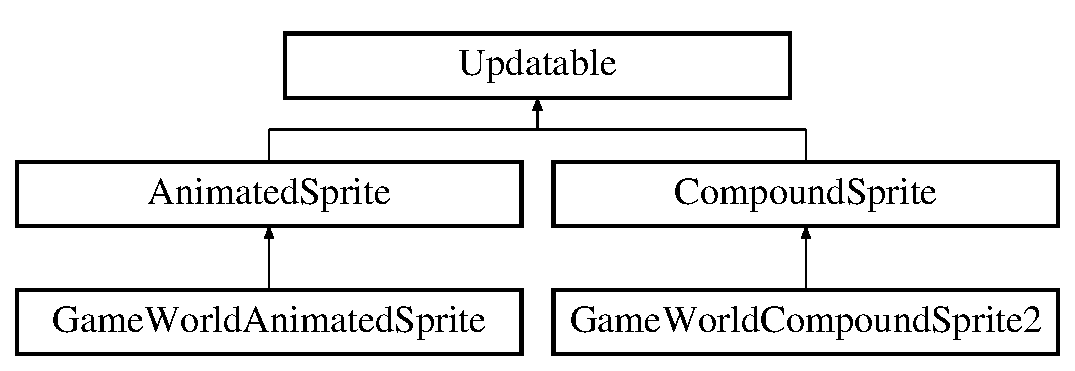
\includegraphics[height=3.000000cm]{class_updatable}
\end{center}
\end{figure}
\subsection*{Public Member Functions}
\begin{DoxyCompactItemize}
\item 
\mbox{\Hypertarget{class_updatable_a60644f5011197f7b371379edeb016fe9}\label{class_updatable_a60644f5011197f7b371379edeb016fe9}} 
virtual void {\bfseries update} (sf\+::\+Time current\+Time)=0
\end{DoxyCompactItemize}
\subsection*{Protected Attributes}
\begin{DoxyCompactItemize}
\item 
\mbox{\Hypertarget{class_updatable_aa34a7210d368ca86c9a49b6cf75aa978}\label{class_updatable_aa34a7210d368ca86c9a49b6cf75aa978}} 
sf\+::\+Time {\bfseries last\+Update}
\end{DoxyCompactItemize}


\subsection{Detailed Description}
Abstract class meant to be inherited. Class that is capable of being updated. 



The documentation for this class was generated from the following file\+:\begin{DoxyCompactItemize}
\item 
E\+:/\+Programing/\+Programing/\+Cpp/\+Game\+Backbone/\+Game\+Backbone/Updatable.\+h\end{DoxyCompactItemize}

%--- End generated contents ---

% Index
\backmatter
\newpage
\phantomsection
\clearemptydoublepage
\addcontentsline{toc}{chapter}{Index}
\printindex

\end{document}
